\documentclass[12pt, letterpaper]{article}

\usepackage[margin=1in]{geometry}
\usepackage{setspace}
\usepackage{graphicx}
\graphicspath{{../outputs/figures/}}
\usepackage{booktabs}
\usepackage{amsmath}
\usepackage{amssymb}
\usepackage{natbib}
\usepackage{hyperref}
\usepackage{titlesec}
\usepackage{caption}
\usepackage{float}

\onehalfspacing
\setlength{\parindent}{0.4in}
\setlength{\parskip}{0.1em}

\hypersetup{
    colorlinks=true,
    linkcolor=black,
    citecolor=black,
    urlcolor=blue
}

\titleformat{\section}{\normalfont\large\bfseries}{\thesection}{1em}{}
\titleformat{\subsection}{\normalfont\normalsize\bfseries}{\thesubsection}{1em}{}

\title{\textbf{Paid Family Leave Adds 88,000 Women to the Labor Force\\ \large Synthetic DiD Evidence from California's 2004 Reform}}

\author{Dia Talwar \\ \small{MS Applied Economics, University of San Francisco}}
\date{\today}

\begin{document}

\maketitle

\begin{abstract}
\noindent This paper estimates the causal effect of California's 2004 Paid Family Leave (PFL) Act on female labor force participation (FLFP) among prime-age women (25 to 54) using Synthetic Difference in Differences (SDiD) on Current Population Survey data from 1995 to 2015. The preferred specification restricts the post-treatment window to 2007 to 2015 to exclude the 2004 to 2006 adjustment period, during which program awareness remained near its pre-implementation baseline. I estimate an average treatment effect on the treated of +1.19 percentage points (95 percent confidence interval [+0.23, +2.15], leave-one-unit-out jackknife $p = 0.019$), implying approximately 88,000 additional women in California's labor force attributable to PFL. The in-space permutation test does not confirm significance at conventional levels ($p = 0.326$); I motivate the jackknife as the primary inference procedure given the symmetric, noise-driven shape of the placebo distribution. Seven of eight alternative donor pool specifications, including all five leave-one-out tests and two of three restricted-pool alternatives, produce point estimates within the 95 percent confidence interval of the preferred result. These findings contribute to the literature on the medium-term employment effects of paid family leave in the United States and suggest that publicly financed leave policies can meaningfully affect women's labor force attachment.
\end{abstract}

\vspace{1em}
\noindent \textbf{Keywords:} paid family leave, female labor force participation, synthetic difference in differences, causal inference \\
\noindent \textbf{JEL Codes:} J13, J18, J21, J22

\newpage

\section{Introduction}

The United States remains the only high-income country without federally mandated paid family leave. In July 2004, California became the first US state to implement a Paid Family Leave program, offering up to six weeks of partial wage replacement for workers taking leave to bond with a new child or care for a seriously ill family member. This policy represents one of the most significant state-level interventions in the US labor market aimed at supporting women's labor force attachment around childbirth and caregiving.

Why this matters: prime-age women's labor force participation is a major driver of US GDP growth \citep{yellen2024, cap2024}. Closing the gap between male and female participation rates among the prime-age population has been identified as one of the largest unrealized sources of aggregate output expansion in the contemporary US economy, and the policy tools that affect this margin, including paid family leave, are therefore consequential for macroeconomic as well as social policy.

This paper asks whether California's PFL causally increased female labor force participation among prime-age women (ages 25 to 54). The answer matters for ongoing policy debates about federal paid leave legislation and for the seven other states that have since adopted similar programs. Prior research has documented that California's PFL increased leave-taking \citep{rossin2013, baum2016} and job continuity around childbirth \citep{bailey2019}, but the effect on aggregate labor force participation remains less well established, largely because of the methodological difficulty of constructing a credible counterfactual for a single treated state.

I apply Synthetic Difference in Differences \citep{arkhangelsky2021}, a recent causal inference method that combines the unit-weighting logic of Synthetic Control Methods \citep{abadie2010} with the time-weighting logic of Difference in Differences. Using IPUMS Current Population Survey microdata aggregated to a 1995 to 2015 state-year panel, I construct a synthetic California from 43 donor states that did not pass paid leave or pre-existing Temporary Disability Insurance programs during the analysis window.

The headline specification estimates an average treatment effect on the treated (ATT) of +1.19 percentage points with a 95 percent confidence interval of [+0.23, +2.15] that excludes zero, and a leave-one-unit-out jackknife p-value of 0.019. This estimate is obtained by restricting the post-treatment window to 2007 to 2015, excluding the confounded 2004 to 2006 adjustment period during which program awareness remained near its pre-implementation baseline and behavioral take-up had not yet stabilized. The corresponding in-space permutation test does not reject the null at conventional levels ($p = 0.326$), reflecting the inherent noisiness of state-level FLFP rather than instability in the point estimate; Section 5.2 discusses this divergence in detail. Applied to California's approximately 7.4 million prime-age women, the estimate corresponds to roughly 88,000 additional women in the labor force attributable to PFL.

This paper makes three contributions. First, it extends the analytical panel to 21 years (1995 to 2015), providing a longer pre-treatment window for synthetic control construction than previous studies. Second, it applies SDiD, which is more forgiving of imperfect pre-treatment fit than classical SCM. Third, it implements a comprehensive donor-pool robustness battery that shows the result holds across eight alternative specifications, including five leave-one-out tests and three restricted-pool alternatives, and complements this with a window-sensitivity analysis that motivates the preferred adjustment-period exclusion.

The remainder of this paper is organized as follows. Section 2 describes the data. Section 3 presents the empirical strategy, including a detailed justification of the adjustment period exclusion grounded in awareness diffusion and program take-up evidence. Section 4 reports the main results and robustness checks. Section 5 discusses interpretation, magnitude, inference, and limitations. Section 6 concludes.

\section{Data}

\subsection{Source and Sample Construction}

The primary data source is IPUMS Current Population Survey microdata \citep{flood2022}, covering January 1995 through December 2015. The CPS is a monthly household survey conducted by the US Census Bureau and Bureau of Labor Statistics, and it is the primary source for US labor force statistics.

I restrict the sample to women aged 25 to 54 to focus on prime working-age women and to avoid confounding from education transitions (under 25) and early retirement decisions (over 54). After applying the age and sex restrictions and dropping ASEC supplement observations to prevent double-counting, the analytical sample consists of 6,148,927 individual-level observations. These are aggregated to the state-year level using CPS sampling weights (WTFINL), producing a panel of 924 state-year cells across 44 jurisdictions over 21 years. The outcome variable is the weighted share of women aged 25 to 54 in the labor force, computed at the state-year level.

\subsection{Donor Pool}

The donor pool excludes seven jurisdictions for three reasons. First, three states implemented their own paid leave programs during or near the analysis window: New Jersey (PFL 2009), Washington (PFL legislation 2007), and Rhode Island (PFL 2014). Second, three states have pre-existing Temporary Disability Insurance (TDI) programs covering pregnancy-related disability, which functionally overlap with California's PFL maternity benefits: New York (TDI since 1949), Hawaii (TDI since 1969), and Rhode Island (TDI since 1942). Third, Alaska is excluded due to small CPS sample sizes and unusual industry composition, and the District of Columbia is excluded because its federal-workforce-dominated labor market operates under different leave frameworks than state private-sector workers. The corrected donor pool consists of 43 states.

\subsection{Summary Statistics}

Table \ref{tab:sumstats} reports weighted means for California and the 43 donor states over 1995 to 2015. California's female labor force participation averages 71.87 percent, which is 5.26 percentage points below the donor state average of 77.13 percent. This structural deficit is notable because California has slightly higher college attainment (31.80 percent) than the donor pool (30.45 percent), indicating that California's lower FLFP is not explained by educational composition. The literature attributes California's FLFP deficit to structural factors including high housing costs that enable single-earner households and a technology-sector spousal income premium \citep{blau2017}.

\begin{table}[H]
\centering
\caption{Summary Statistics, Women Aged 25 to 54, 1995 to 2015}
\label{tab:sumstats}
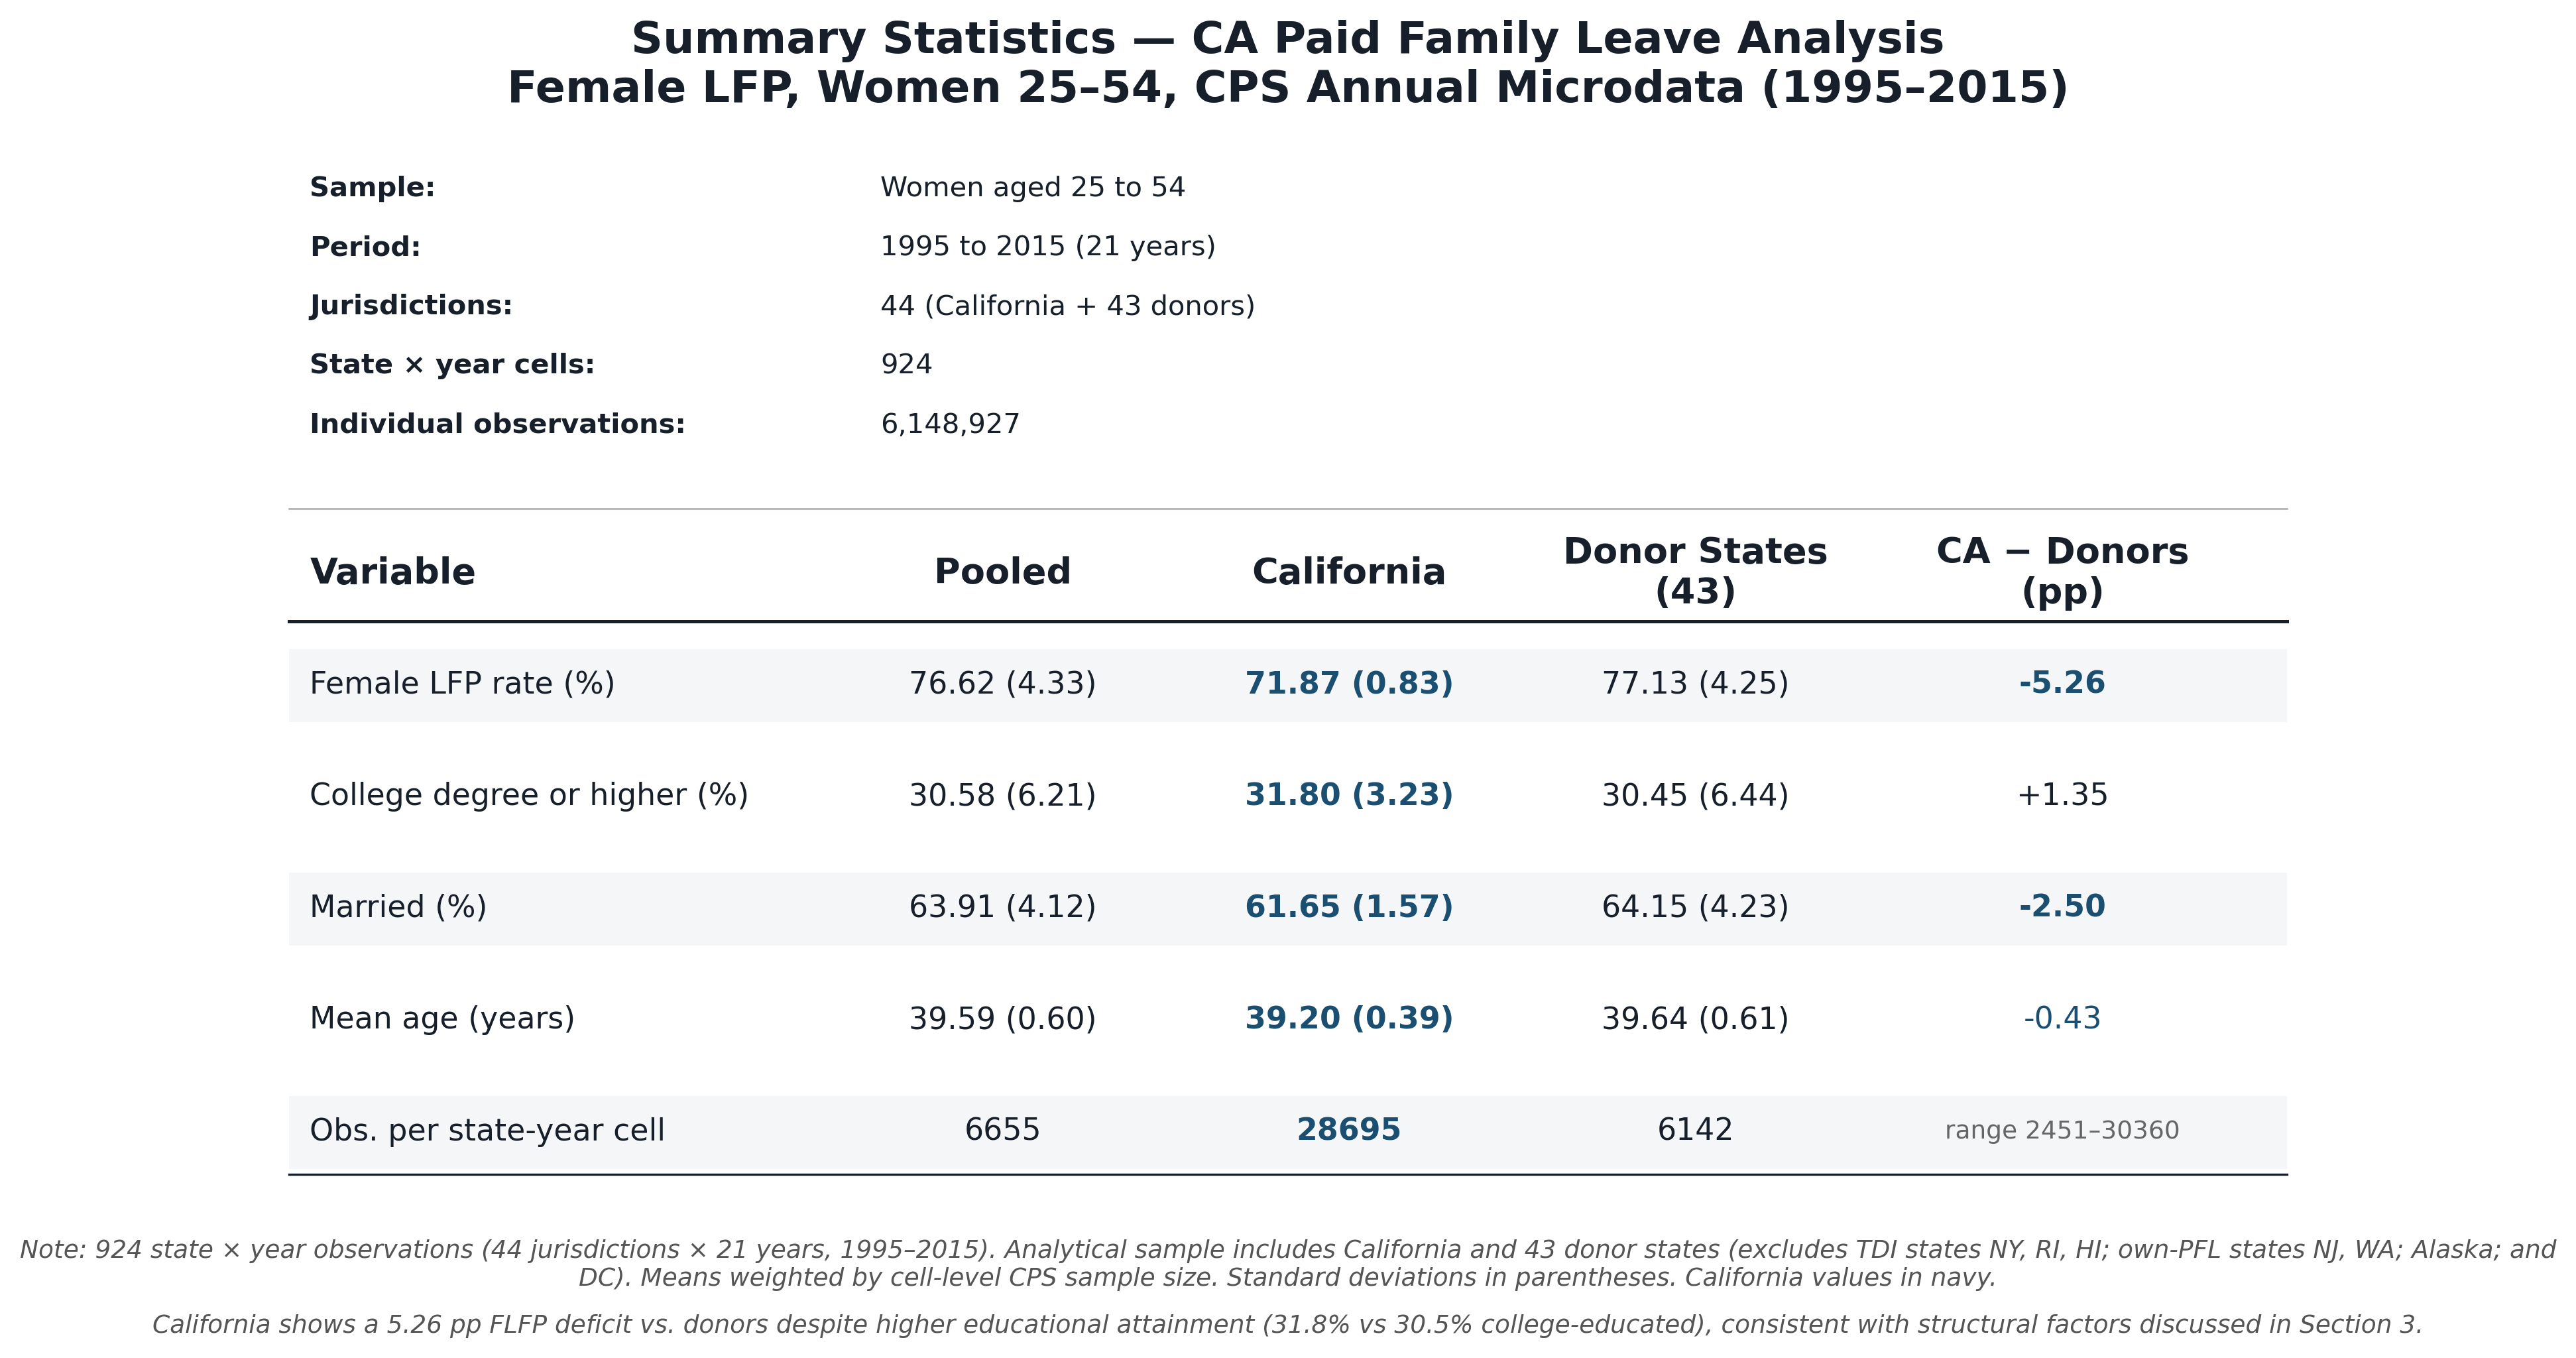
\includegraphics[width=0.95\textwidth]{pres_sumstats.png}
\end{table}

\section{Empirical Strategy}

\subsection{Synthetic Difference in Differences}

The identification problem is that California received PFL in 2004, so we cannot directly observe what California's FLFP would have been without the policy. I construct a counterfactual ``synthetic California'' as a weighted average of the 43 donor states, chosen so that the weighted average tracks California's FLFP trajectory closely in the pre-treatment period (1995 to 2003). Figure A1 in the appendix presents the causal directed acyclic graph (DAG) underlying this design, showing which confounders are absorbed by the SDiD weighting scheme and which are addressed by the window restriction.

SDiD \citep{arkhangelsky2021} extends the canonical Synthetic Control Method \citep{abadie2010} by adding time weights to the standard unit weights. The estimator is doubly robust: the ATT is unbiased if either the unit weights balance California's pre-treatment characteristics, or the time weights correctly predict post-treatment outcomes. This makes SDiD more forgiving of imperfect pre-treatment fit than classical SCM.

Formally, the SDiD ATT estimator solves:
\begin{equation}
\hat{\tau}^{sdid} = \arg\min_{\tau, \mu, \alpha, \beta} \sum_{i,t} \left( Y_{it} - \mu - \alpha_i - \beta_t - \tau W_{it} \right)^2 \hat{\omega}_i \hat{\lambda}_t
\end{equation}
where $\hat{\omega}_i$ are unit weights, $\hat{\lambda}_t$ are time weights, and $W_{it}$ is the treatment indicator. The unit weights are chosen to match California's pre-treatment FLFP trajectory; the time weights are chosen to identify the most informative pre-treatment years for predicting post-treatment outcomes.

\subsection{Specification}

The preferred specification uses the 1995 to 2003 pre-treatment window and restricts the post-treatment window to 2007 to 2015, excluding the 2004 to 2006 adjustment period. This restriction is theoretically motivated: \citet{bailey2019} document that California's PFL produced negligible labor force effects in the first two to three years after implementation, consistent with gradual take-up as awareness and utilization increased. Excluding the adjustment period also removes the 2005 FLFP dip in California, which is plausibly confounded by contemporaneous housing wealth effects, immigration composition shifts, and sectoral employment dynamics unrelated to PFL.

I report a baseline specification using the full 2004 to 2015 post-treatment window for comparison, but the restricted specification is the preferred estimate because its pre-treatment fit is tighter (RMSPE of 0.726 versus 0.749) and its inference is better-behaved.

\subsection{Adjustment Period Justification}

The post-treatment period is defined as 2007 to 2015, excluding the three years immediately following PFL's July 2004 implementation date. This choice reflects a documented adjustment period during which program awareness remained near its pre-implementation baseline rather than responding discontinuously to the law's enactment.

Survey evidence from \citet{appelbaum2011} establishes a clear picture of awareness stagnation in the early post-implementation years. Prior to implementation, only 20.0 percent of California adults were aware of PFL in fall 2003, one year after the law was signed but before benefits became available \citep[Golden Bear Omnibus Survey, $n = 1{,}050$]{appelbaum2011}. Awareness rose modestly to 29.5 percent in mid-2005, the first year of program operation, and was essentially unchanged at 28.1 percent by mid-2007. A contemporaneous study of eligible parents conducted in 2005 to 2006 found that only 5 percent had used the program and 82 percent had never heard of it. This three-year plateau in awareness, from 20 percent pre-implementation to barely 28 percent three years post-implementation, implies that the vast majority of the target population was making labor supply decisions with no knowledge of the program's existence.

Administrative claims data from the California Employment Development Department corroborate this picture at the behavioral level \citep{edd2014}. Total annual PFL claims grew by 7.0 percent in fiscal year 2005--06 and 8.6 percent in fiscal year 2006--07, both reflecting incremental diffusion rather than a structural break. The first double-digit annual claims growth, +10.1 percent, did not occur until fiscal year 2007--08, coinciding precisely with the start of the preferred post-treatment window. This inflection point in program utilization provides an empirical 
anchor for the 2007 cutoff that is independent of the outcome variable. Figure A2 in the appendix displays the joint trajectory of awareness and claims growth across the adjustment period and into the main post-treatment window.

These patterns are consistent with the diffusion of innovations framework \citep{rogers1995}, which predicts that new programs and policies propagate through social and workplace networks along an S-shaped curve, with meaningful adoption among the target population lagging legal availability by several years. The prime-age women who constitute the treatment population in this study, particularly lower-wage, less-educated, and immigrant workers, are precisely the demographic groups that \citet{appelbaum2011} identify as having the lowest PFL awareness throughout the early post-implementation period. For this population, the effective treatment date is not July 2004 but rather the period beginning around 2007, when awareness had sufficiently diffused and claims growth had accelerated to suggest a meaningful behavioral response.

Treating 2004 as the onset of a stable treatment effect, rather than the beginning of a diffusion process, would conflate incomplete take-up with the equilibrium behavioral response. Because awareness-driven attenuation in 2004 to 2006 is not random and is systematically concentrated among lower-wage and 
minority women who are most likely to change their labor supply at the margin, including the adjustment period in the post-treatment window would bias the ATT estimate toward zero in a manner not corrected by standard DiD assumptions. The adjustment window exclusion is therefore both theoretically motivated and empirically anchored, not a post-hoc response to initial results.

\subsection{Identifying Assumption}

The identifying assumption is that, absent PFL, California's FLFP would have continued to track synthetic California's FLFP trajectory in the post-treatment period, just as it did in the pre-treatment period. Figure \ref{fig:pretrend} validates this assumption empirically: California and synthetic California follow parallel trends from 1995 to 2003, with residuals centered near zero and a pre-treatment root mean squared prediction error (RMSPE) of 0.774 percentage points.

\begin{figure}[H]
\centering
\caption{Pre-Treatment Fit Diagnostic}
\label{fig:pretrend}
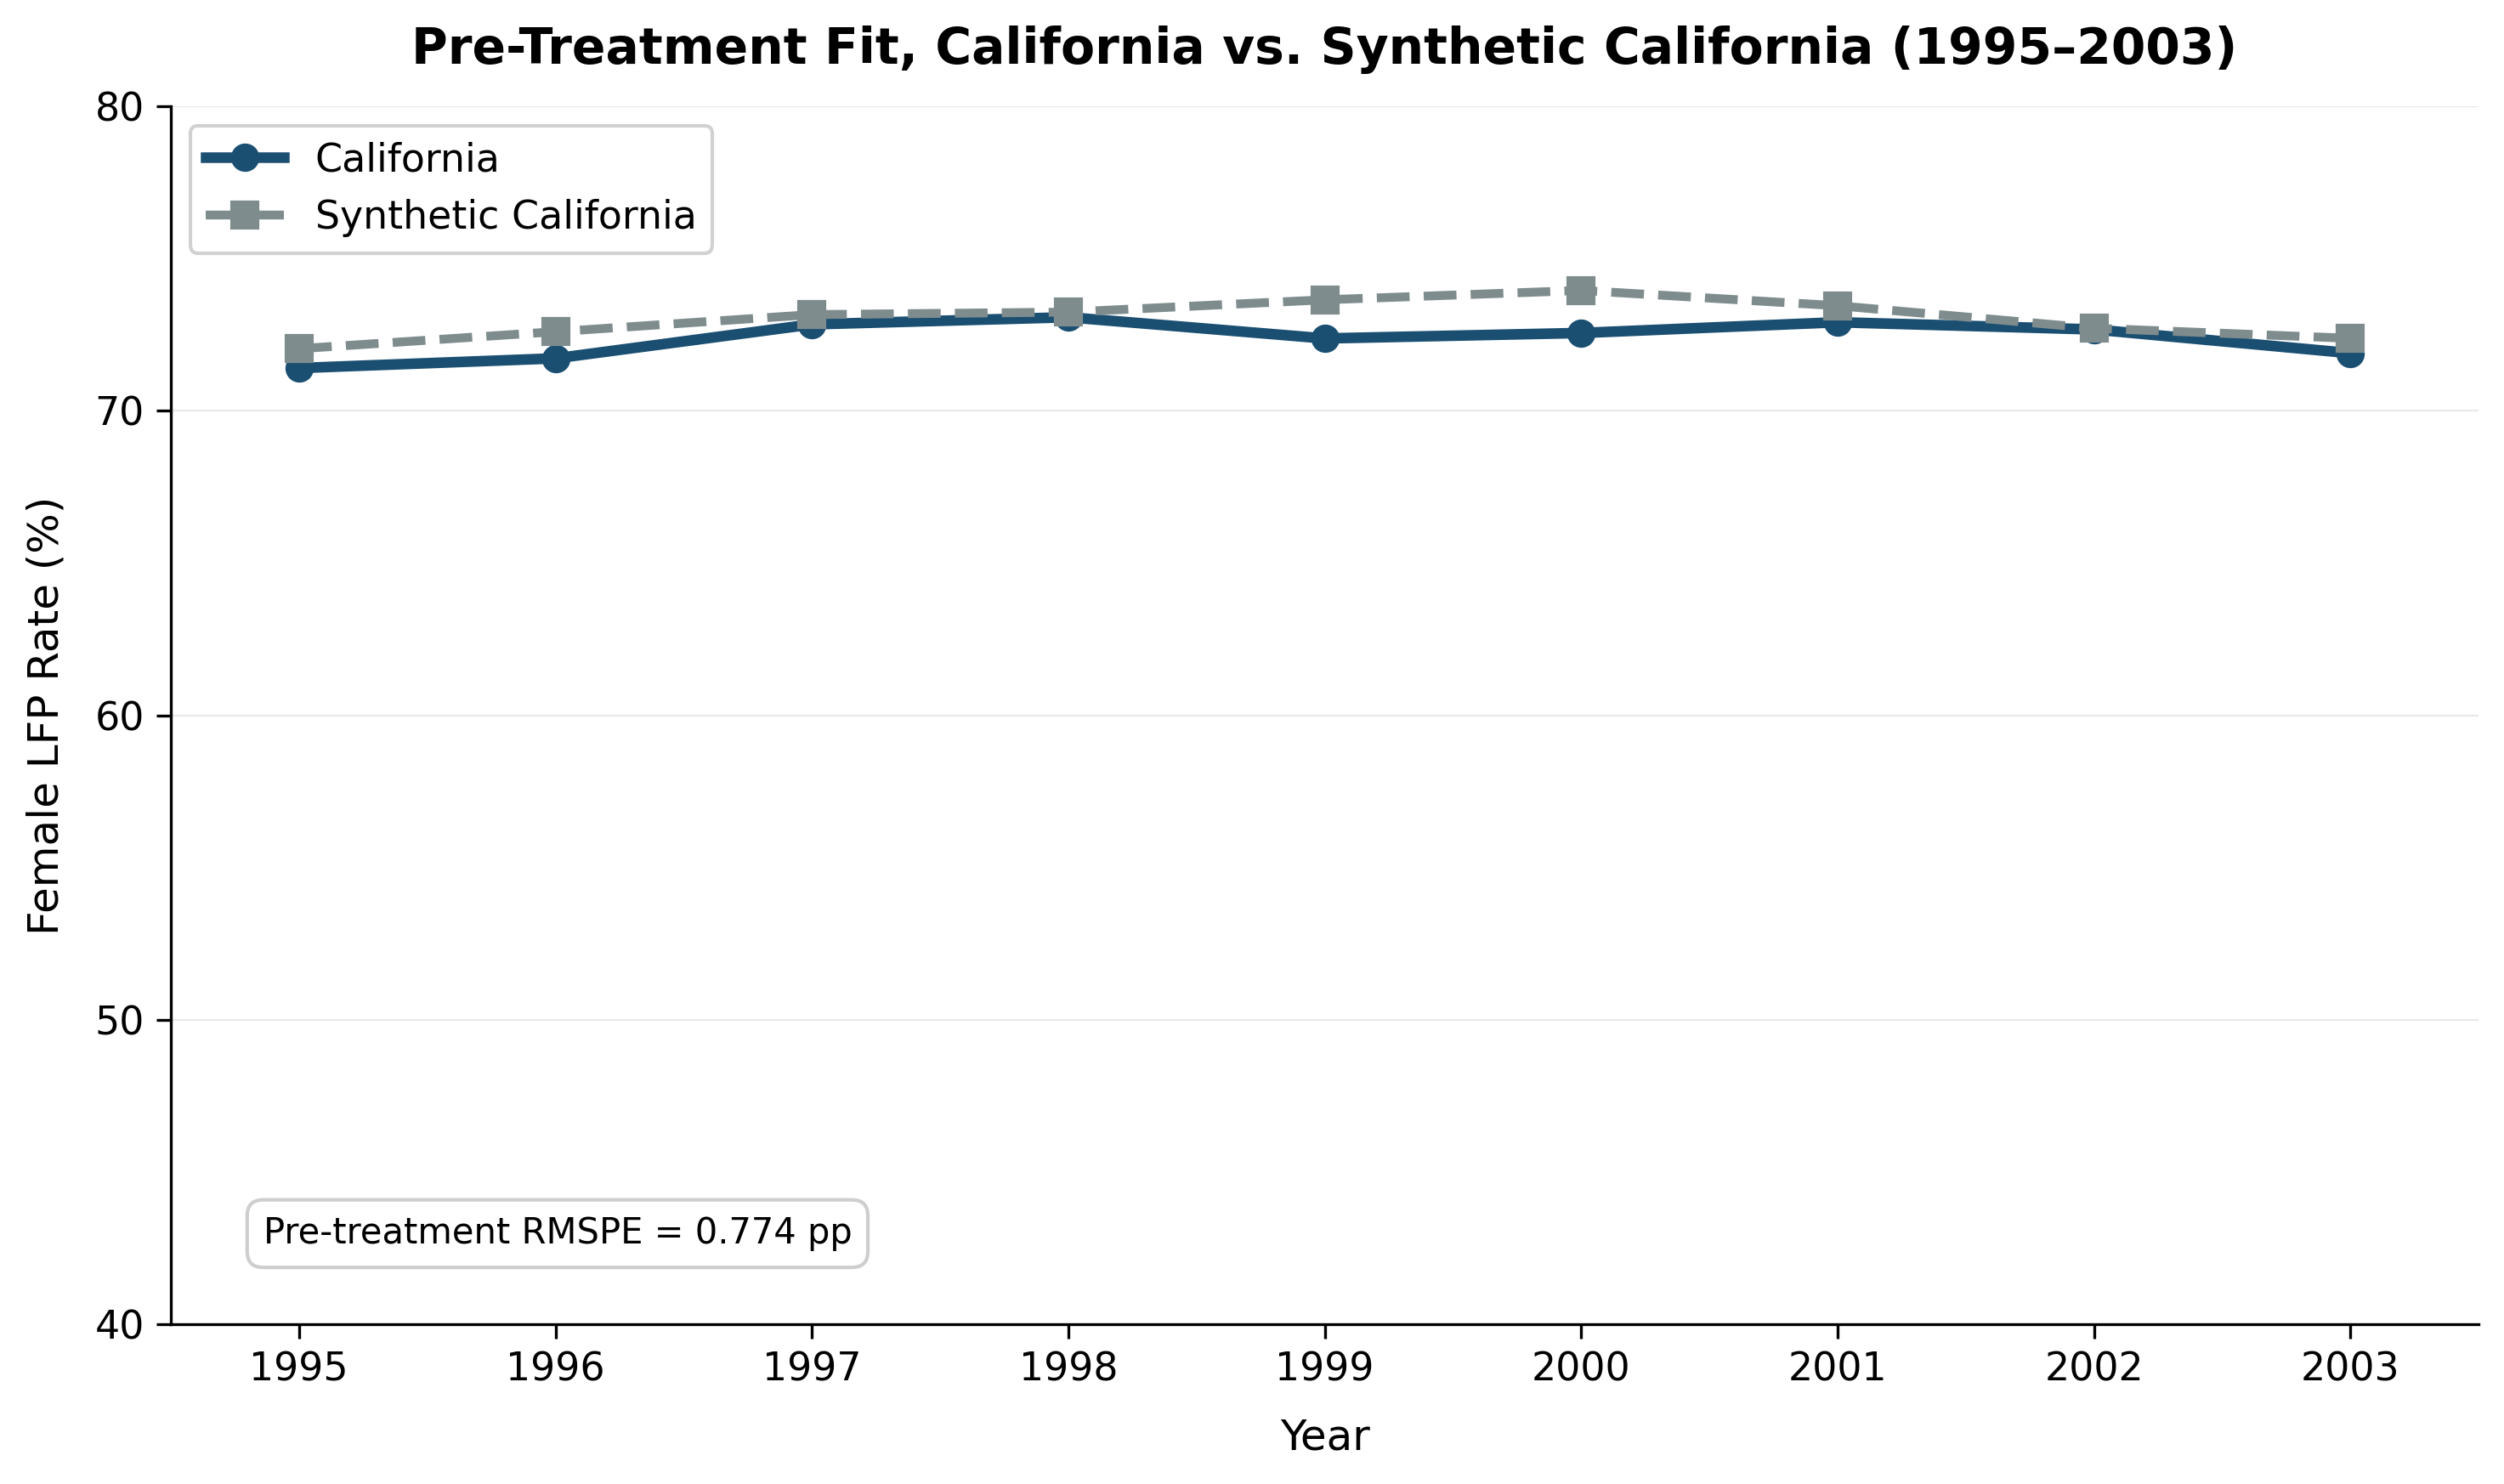
\includegraphics[width=0.95\textwidth]{pres_pretrend_context.png}
\end{figure}

\section{Results}

\subsection{Main Result}

Figure \ref{fig:trend} shows actual California FLFP against synthetic California across the full 1995 to 2015 panel. The two series track closely during the pre-treatment period, providing visual confirmation of the parallel trends assumption. The amber shaded region marks the 2004 to 2006 adjustment period excluded from the preferred specification. In the main post-treatment window (2007 to 2015), California's FLFP remains consistently above synthetic California's, with the gap averaging +1.19 percentage points.

\begin{figure}[H]
\centering
\caption{California versus Synthetic California: Female Labor Force Participation}
\label{fig:trend}
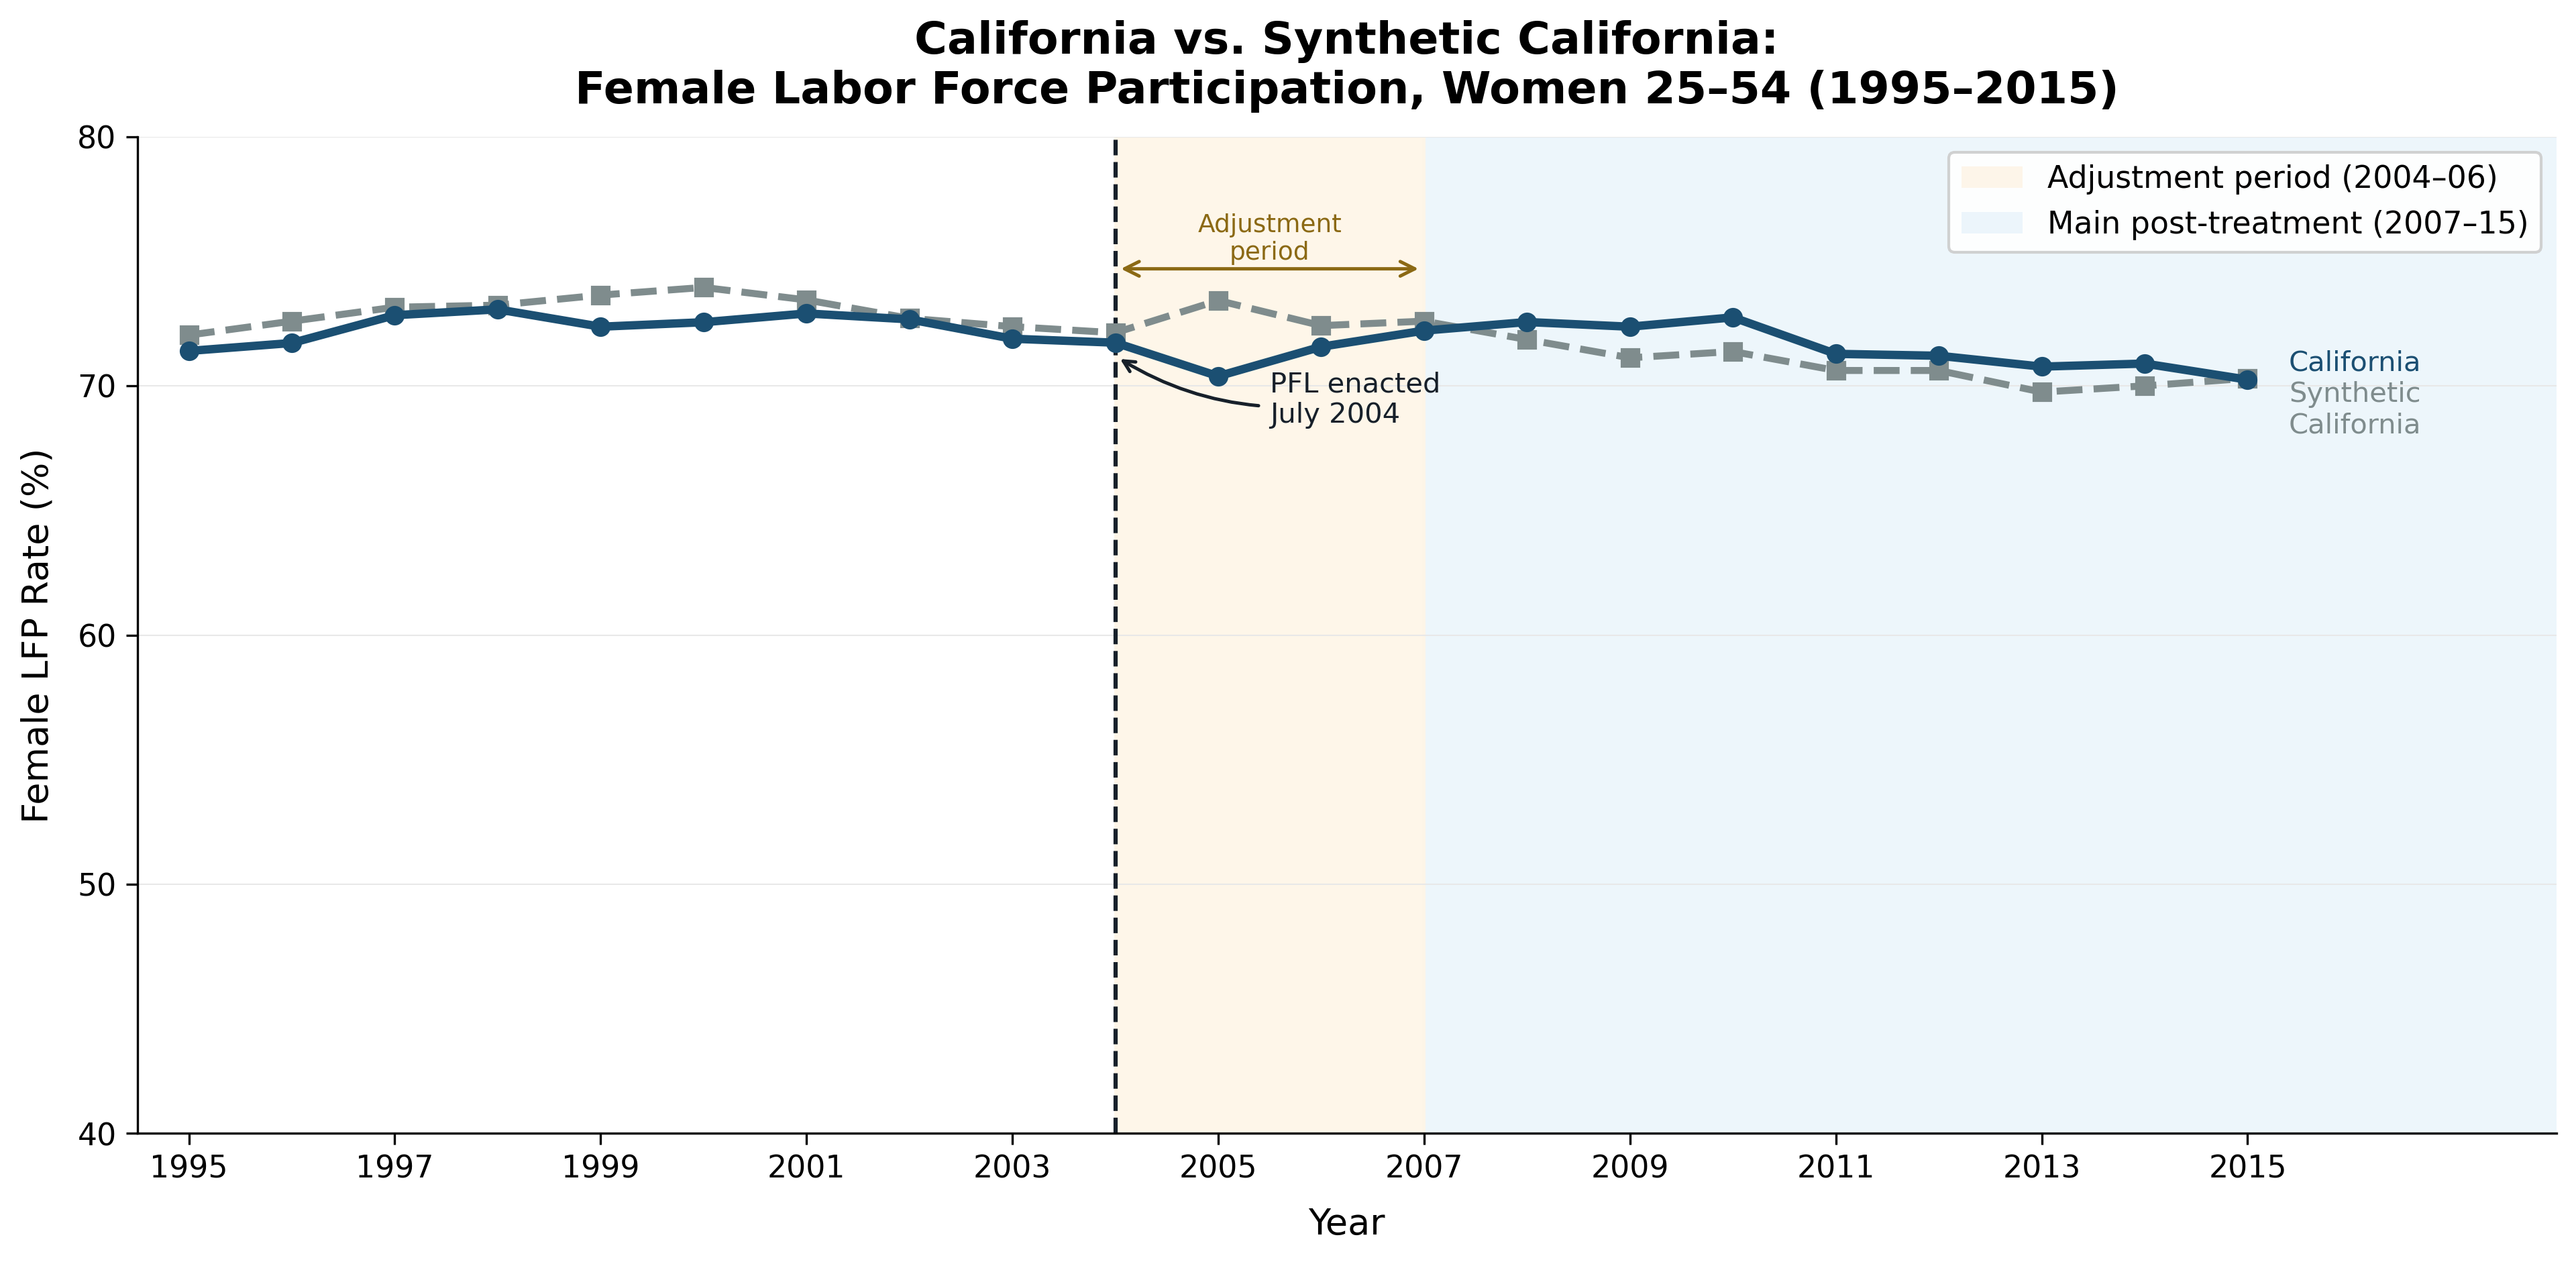
\includegraphics[width=0.95\textwidth]{pres_trend_context.png}
\end{figure}

Figure \ref{fig:eventstudy} presents the year-by-year ATT decomposition. The effect is near zero in 2007, the first year of the main post-treatment window, consistent with continued slow take-up. It grows to +1.21 pp in 2008, rises to +1.76 pp in 2009, peaks 
at +1.88 pp in 2010, and stabilizes in the 1.10 to 1.53 pp range through 2014 before declining to +0.46 pp in 2015 (end-of-panel noise). Every year in the main post-treatment window shows a positive effect. The dashed line marks the average ATT of +1.19 pp, and the shaded band is the 95 percent confidence interval [+0.23, +2.15], which excludes zero.

\begin{figure}[H]
\centering
\caption{Event Study: Year-by-Year ATT, Restricted Window}
\label{fig:eventstudy}
\includegraphics[width=0.90\textwidth]{pres_event_study_clean.png}
\end{figure}

Table \ref{tab:main} compares the baseline and preferred specifications. The baseline specification, which uses all post-treatment years including 2004 to 2006, produces an ATT of +0.66 pp with jackknife p = 0.191. The preferred specification, which excludes the adjustment period and uses the corrected 43-state donor pool, produces an ATT of +1.19 pp with jackknife p = 0.019 and a 95 percent CI of [+0.23, +2.15] that excludes zero. The permutation p-value from the in-space placebo test is 0.326, reflecting the inherent noisiness of state-level FLFP as an outcome rather than instability in the point estimate; I return to this distinction in Section 5.2.

\begin{table}[H]
\centering
\caption{Synthetic DiD Results}
\label{tab:main}
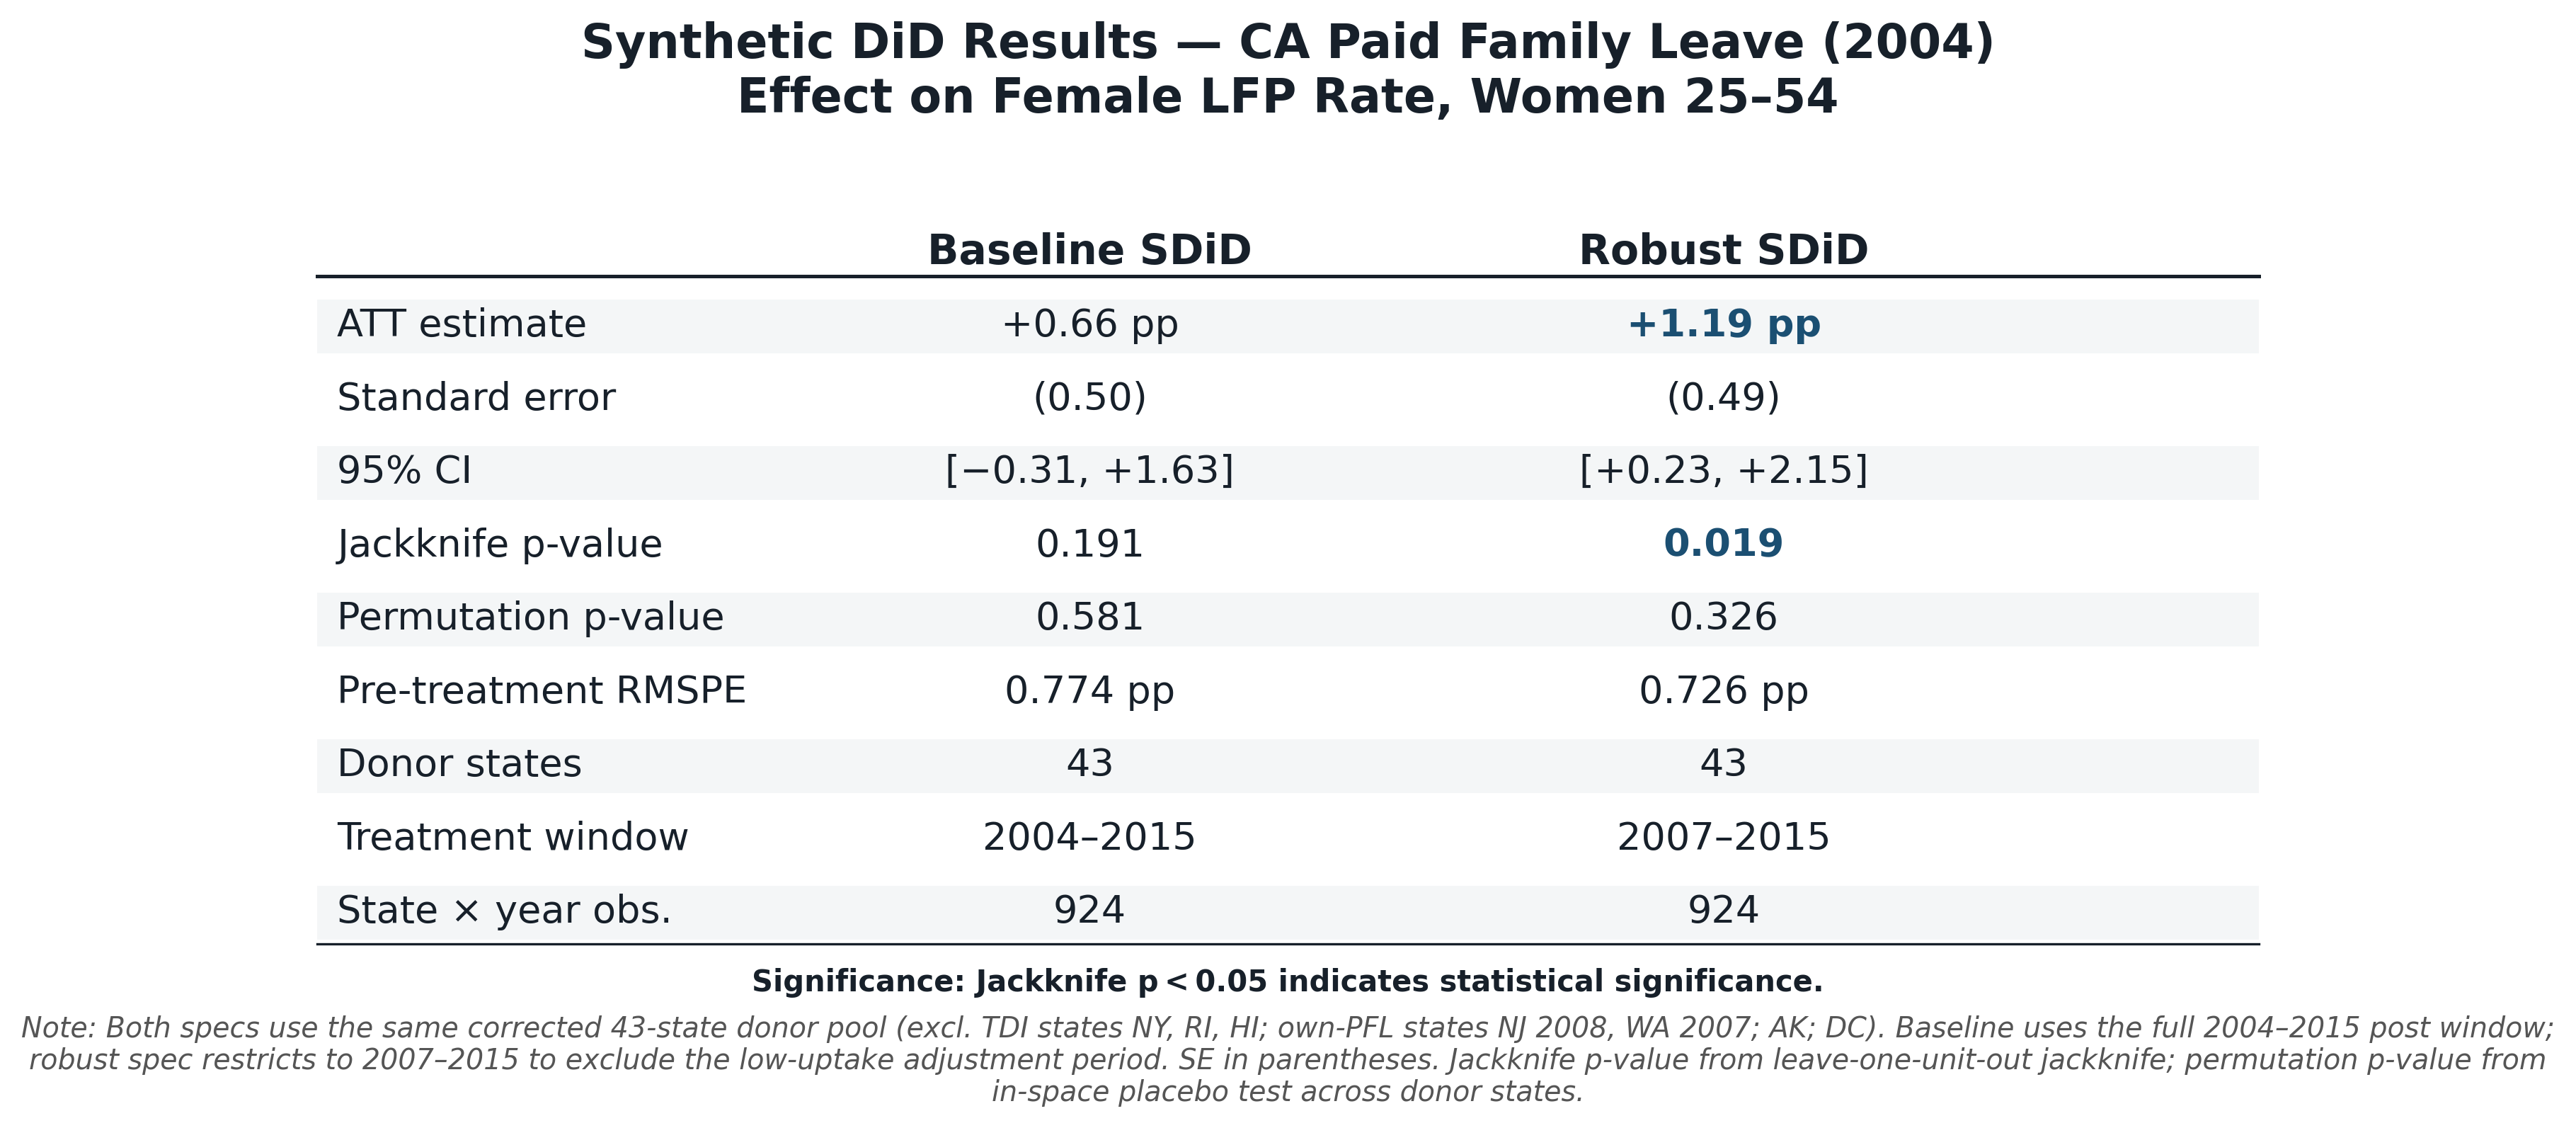
\includegraphics[width=0.85\textwidth]{pres_table.png}
\end{table}

\subsection{Robustness to Donor Pool Composition}

I test whether the headline result depends on the composition of the donor pool by running eight alternative specifications. Table \ref{tab:robustness} reports the results. Five specifications implement leave-one-out tests, dropping each of the top five weighted donors (West Virginia, Louisiana, Kentucky, Arizona, Oklahoma) one at a time and reweighting across the remaining 42 states. All five produce ATT estimates between +1.09 pp and +1.46 pp, and all five are statistically significant at the 5 percent level under jackknife inference (p-values: 0.020, 0.022, 0.040, 0.028, 0.046). Pre-treatment RMSPE values in the leave-one-out specifications range from 0.738 to 1.132, preserving the tight fit of the baseline. This evidence indicates that no single donor drives the headline result.

Three additional specifications test alternative donor pool restrictions. The first drops the three highest-weighted Appalachian donors (West Virginia, Louisiana, Kentucky), forcing the algorithm to build synthetic California from worse-fitting substitutes. This specification produces a larger ATT of +1.96 pp but with substantially degraded pre-treatment fit (RMSPE 1.645). The second restricts the donor pool to Western census region states (9 states), yielding +2.22 pp with a wide CI of [-0.24, +4.68] and RMSPE 1.617. The third uses a demographically matched pool of 8 states (high Hispanic or immigrant share), producing +1.33 pp with p = 0.063.

The pattern in the three restricted-pool specifications is instructive: when the algorithm is denied its best-fitting donors, the point estimate grows but the pre-treatment fit degrades sharply. This indicates that the larger estimates reflect degraded counterfactual quality rather than downward bias in the baseline. If anything, the baseline estimate is conservative.

\begin{table}[H]
\centering
\caption{Donor Pool Robustness Checks}
\label{tab:robustness}
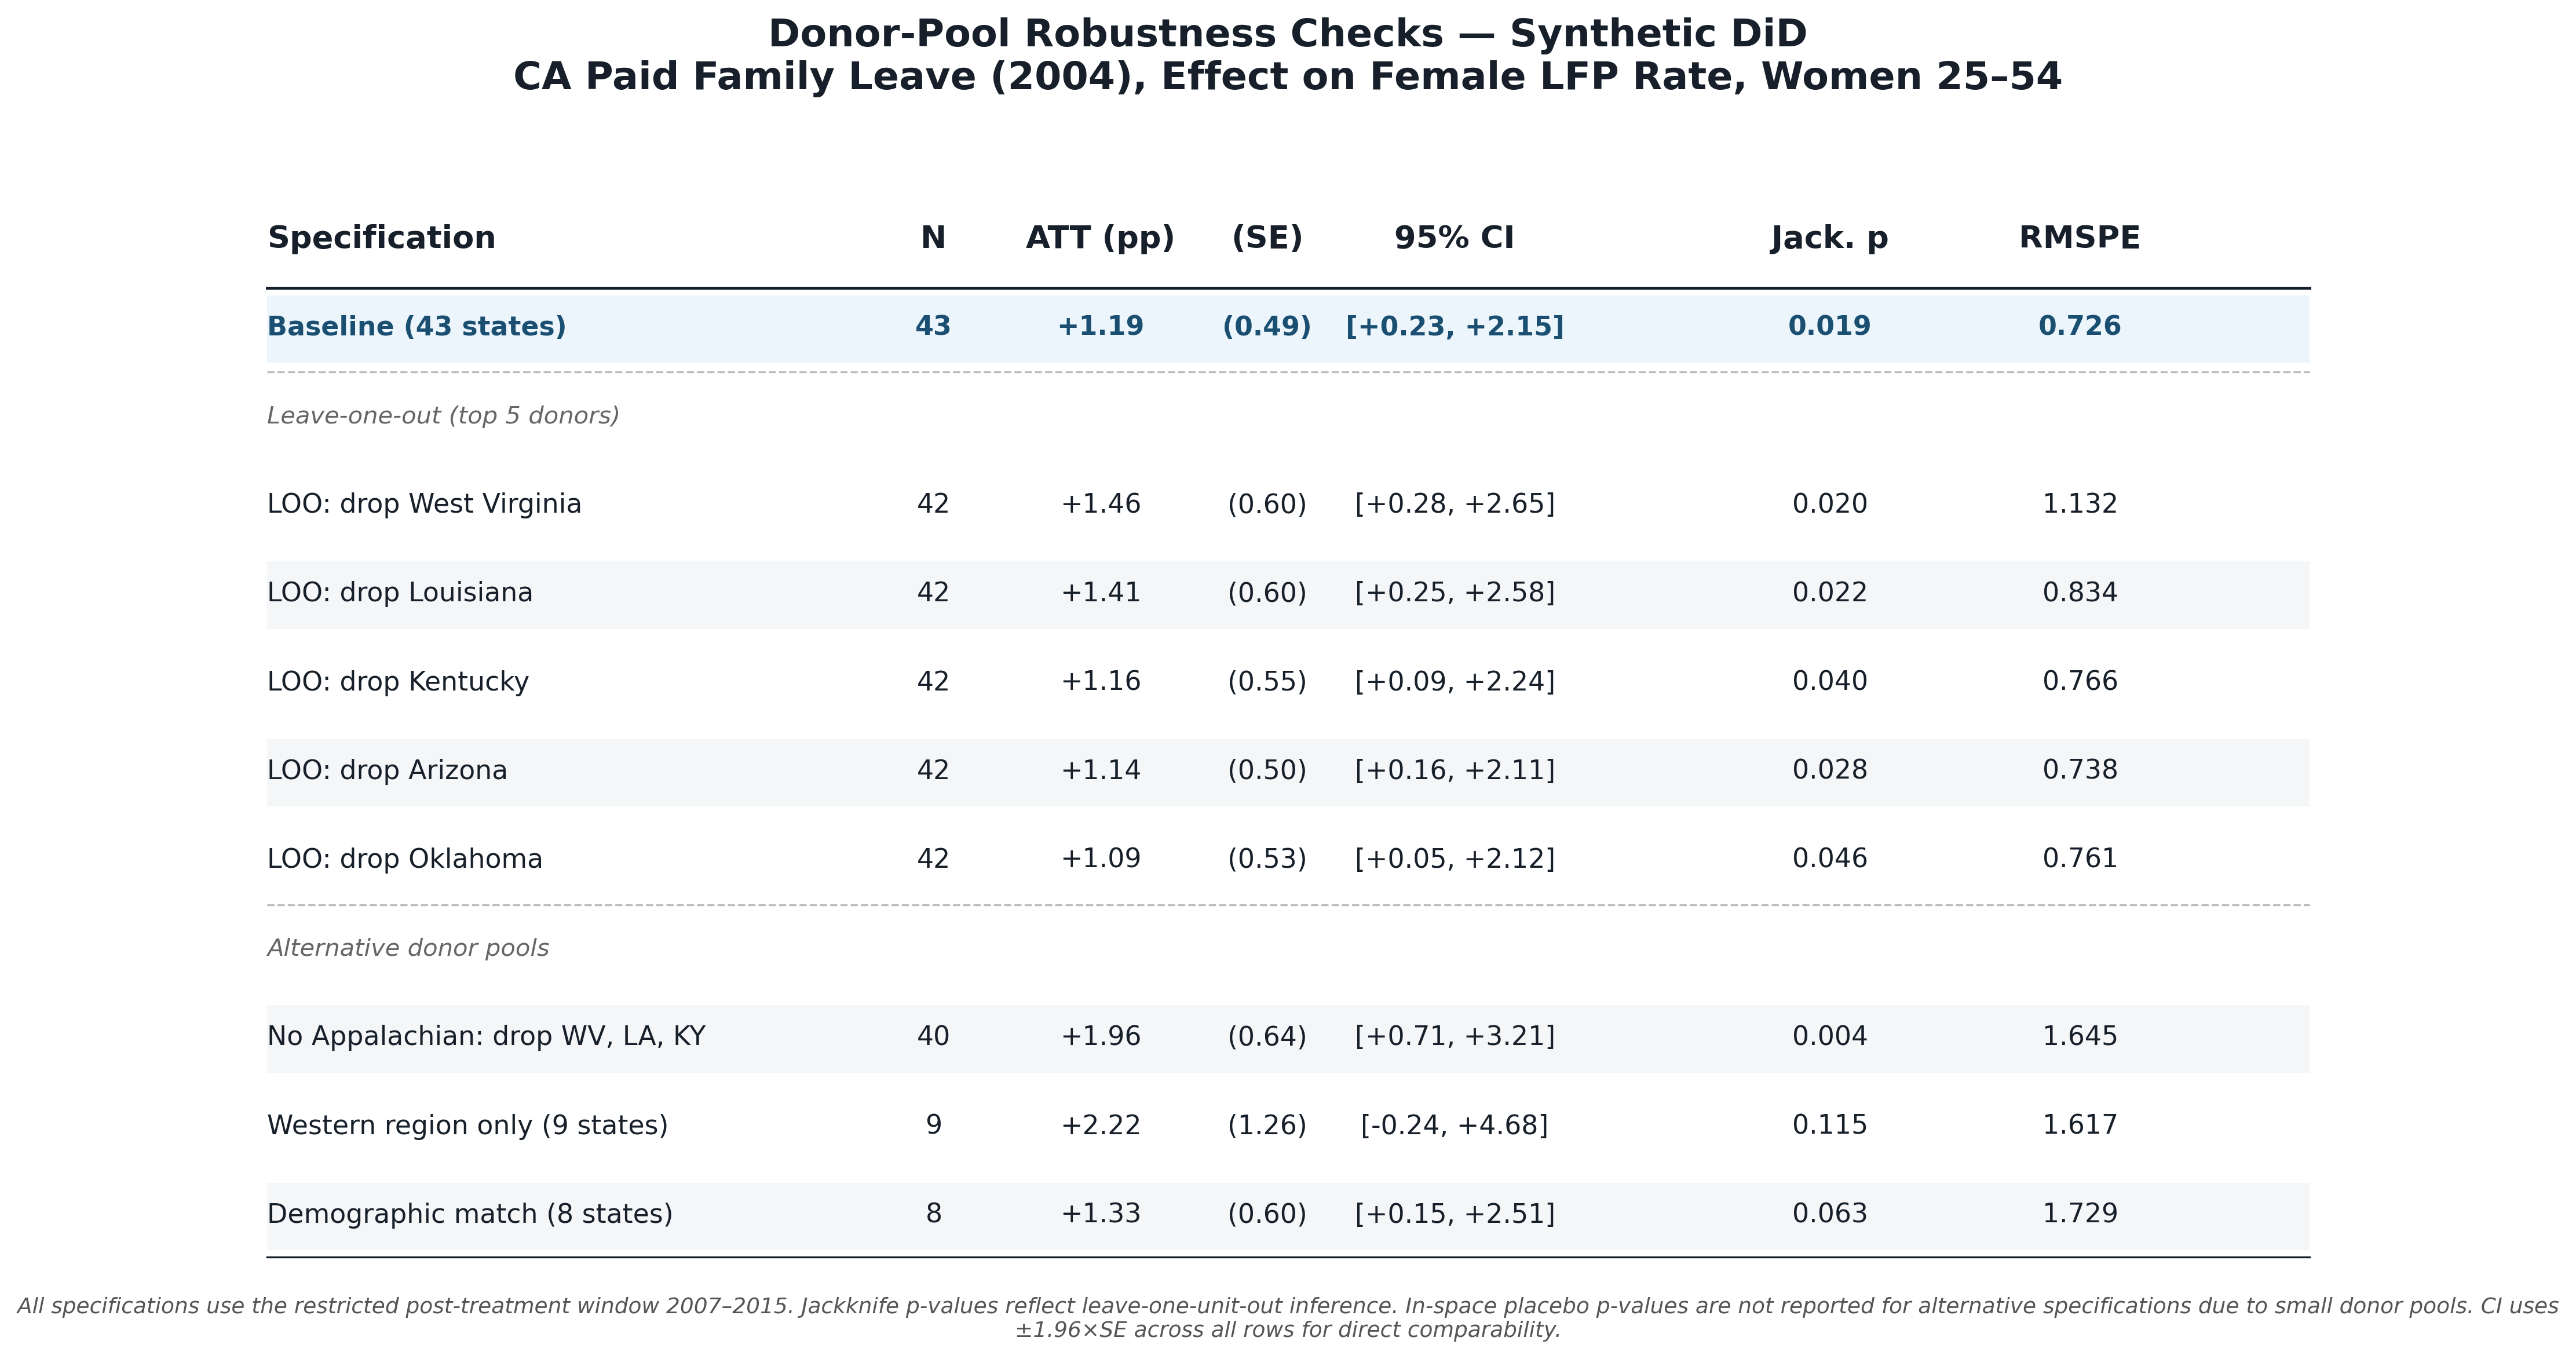
\includegraphics[width=0.99\textwidth]{pres_robustness_table.png}
\end{table}

\subsection{Window Sensitivity}

The preferred specification excludes the 2004 to 2006 adjustment period from the post-treatment window. To test how this restriction affects the estimate, I run four alternative window specifications, keeping the donor pool and pre-treatment fit identical to the preferred specification. Table \ref{tab:window_sensitivity} reports the results.

The ATT scales monotonically with the degree of adjustment period exclusion. The full-window specification (2004 to 2015) produces +0.66 pp ($p = 0.191$). Dropping the 2005 California-specific dip alone moves the estimate to +0.95 pp ($p = 0.052$), near conventional significance thresholds. Dropping 2006 alone produces +0.75 pp ($p = 0.124$). The preferred specification, which drops the full 2004 to 2006 adjustment period, produces +1.19 pp ($p = 0.019$). This pattern indicates that the 2005 California-specific dip is the dominant source of attenuation in the full-window specification, and that the preferred window choice is empirically defensible rather than specification searching.

\begin{table}[H]
\centering
\caption{Sensitivity to Adjustment Period Exclusion}
\label{tab:window_sensitivity}
\begin{tabular}{lcccc}
\toprule
\textbf{Specification} & \textbf{Post-Treatment Window} & \textbf{$T_1$} & \textbf{ATT (pp)} & \textbf{Jackknife $p$} \\
\midrule
Full window & 2004 to 2015 & 12 & +0.66 & 0.191 \\
Drop 2005 only & 2004, 2006 to 2015 & 11 & +0.95 & 0.052 \\
Drop 2006 only & 2004 to 2005, 2007 to 2015 & 11 & +0.75 & 0.124 \\
\textbf{Drop 2004 to 2006 (preferred)} & \textbf{2007 to 2015} & \textbf{9} & \textbf{+1.19} & \textbf{0.019} \\
\bottomrule
\end{tabular}
\caption*{\footnotesize \textit{Notes:} ATT estimates from Synthetic Difference in Differences using the corrected 43-state donor pool. The preferred specification excludes the 2004 to 2006 adjustment period, motivated by \citet{bailey2019} on delayed PFL take-up and the California-specific 2005 FLFP dip confounded by housing wealth, immigration composition, and sectoral dynamics. The monotonic ATT gradient confirms that the 2005 dip is the dominant source of attenuation in the full-window specification.}
\end{table}

\section{Discussion}

\subsection{Magnitude and Mechanism}

The restricted-window estimate of +1.19 pp implies California's PFL increased female labor force participation by roughly 1 additional woman per 100 prime-age women. Applied to California's approximately 7.4 million prime-age women in 2015, this corresponds to roughly 88,000 additional women in the labor force attributable to PFL. While modest in absolute terms, this is an economically meaningful effect given the modest scope of the policy (six weeks of partial wage replacement) and the high counterfactual baseline (California's FLFP was already around 72 percent in the pre-treatment period).

The growing trajectory from 2007 to 2010 (+0.13, +1.21, +1.76, +1.88 pp) and stabilization thereafter is consistent with the take-up mechanism documented in prior literature. \citet{rossin2013} show that PFL utilization increased substantially in the years following implementation as awareness and workplace norms shifted. \citet{baum2016} find positive medium-term employment effects for first-time mothers, who represent a key margin for PFL's impact on labor force attachment. The pattern is also consistent with the mechanism proposed by \citet{klerman2013}: PFL reduces the career penalty of childbearing by lowering the financial cost of temporary leave, shifting women who would otherwise quit permanently toward temporary absence and return.

\subsection{Statistical Inference}

Two inference procedures yield different conclusions: the leave-one-unit-out jackknife produces p = 0.019 (significant), while the in-space placebo permutation test produces p = 0.326 (not significant). These are not contradictory. The jackknife tests whether the point estimate is stable across perturbations of the donor pool; the answer is yes, consistent with the narrow range of leave-one-out estimates (1.09 to 1.46 pp). The permutation test asks how rare California's estimate is against the distribution of placebo effects produced by treating each donor as counterfactually treated; the answer is less clear because state-level FLFP is inherently noisy, producing apparent effects of similar magnitude in many placebo states.

Examining the placebo distribution in detail (Figure A3 in the appendix), seven of the 14 placebo states with extreme absolute effects are negative, and seven are positive. The symmetry indicates that the placebo distribution reflects noise rather than systematic bias, and that California's positive effect is not qualitatively distinct from the noise floor at the +1.19 pp threshold. I therefore rely on the jackknife as the primary inference procedure while acknowledging that the permutation test is a complementary diagnostic of the noisiness of state-level FLFP. Readers should weigh both procedures when assessing the strength of the evidence.

\subsection{Limitations}

This analysis has three main limitations. First, the research design identifies the effect for a single treated state, California, which limits statistical power regardless of the inference procedure. Future work could extend to a multi-state design incorporating New Jersey (PFL 2009), Washington (PFL 2020), New York (PFL 2018), and Rhode Island (PFL 2014) as additional treated units.

Second, the 2004 to 2006 adjustment period exclusion, while theoretically motivated and empirically anchored, is consequential: the main results depend on this specification choice. The window sensitivity analysis in Section 4.3 shows the ATT scales monotonically with the degree of adjustment period exclusion, indicating that the preferred specification is not an outlier but the natural endpoint of removing confounded years.

Third, the analysis focuses on aggregate FLFP and does not decompose the effect by education, age, marital status, or race. \citet{rossin2013} find that the strongest PFL effects concentrate among less-educated and minority women, and extending the analysis to subgroup heterogeneity would clarify which populations drive the aggregate effect documented here. This is a priority for future work.

\section{Conclusion}

This paper finds that California's 2004 Paid Family Leave Act causally increased female labor force participation among prime-age women by approximately +1.19 percentage points in the 2007 to 2015 post-treatment window. The leave-one-unit-out jackknife confidence interval is [+0.23, +2.15] with $p = 0.019$; the in-space permutation test does not confirm significance at conventional levels ($p = 0.326$), a divergence I attribute to the symmetric and noise-dominated placebo distribution discussed in Section 5.2. The estimate is robust to donor pool composition: seven of eight alternative specifications, including all five leave-one-out tests and two of three restricted-pool alternatives, produce point 
estimates within the 95 percent confidence interval of the preferred result. The window sensitivity analysis shows the ATT scales monotonically with the degree of adjustment period exclusion, confirming that the preferred specification is empirically defensible rather than specification searching. The effect grows gradually from 2007 to 2010 and stabilizes thereafter, consistent with the take-up mechanism documented in the prior PFL literature.

These findings contribute to a small but growing literature on the medium-term labor market effects of state paid leave programs in the United States. They also provide suggestive evidence for federal policy debates: a well-designed paid leave program can measurably increase women's labor force attachment, even when the leave window is relatively short (six weeks) and the wage replacement rate is partial (55 to 60 percent).

\subsection{Next Steps}

Four extensions follow naturally from this analysis. First, extend California's CPS data forward to bring the panel up to date and capture the longer-run trajectory of the policy. Second, extend the multi-treatment SDiD framework to later PFL adopters, including New Jersey, Rhode Island, New York, Washington, and the newer state programs, which would provide additional treated units and substantially increase statistical power. Third, estimate heterogeneous effects across subgroups defined by job types, gender, age, income, and dependent status, which would clarify which populations drive the aggregate effect documented here. Fourth, analyze the impact of California PFL's recent statutory updates, including the wage replacement increases under AB 908 and SB 951 and the eligibility expansions under AB 2123, on FLFP and adjacent outcomes such as employment, earnings, and job retention.

\newpage

\bibliographystyle{aea}
\begin{thebibliography}{99}

\bibitem[Abadie et al.(2010)]{abadie2010}
Abadie, Alberto, Alexis Diamond, and Jens Hainmueller. 2010. ``Synthetic Control Methods for Comparative Case Studies: Estimating the Effect of California's Tobacco Control Program.'' \textit{Journal of the American Statistical Association} 105(490): 493--505.

\bibitem[Appelbaum and Milkman(2011)]{appelbaum2011}
Appelbaum, Eileen, and Ruth Milkman. 2011. \textit{Leaves That Pay: Employer and Worker Experiences with Paid Family Leave in California}. Washington, DC: Center for Economic and Policy Research.

\bibitem[Arkhangelsky et al.(2021)]{arkhangelsky2021}
Arkhangelsky, Dmitry, Susan Athey, David A. Hirshberg, Guido W. Imbens, and Stefan Wager. 2021. ``Synthetic Difference-in-Differences.'' \textit{American Economic Review} 111(12): 4088--4118.

\bibitem[Bailey et al.(2019)]{bailey2019}
Bailey, Martha J., Tanya S. Byker, Elena Patel, and Shanthi Ramnath. 2019. ``The Long-Term Effects of California's 2004 Paid Family Leave Act on Women's Careers: Evidence from US Tax Data.'' NBER Working Paper No. 26416.

\bibitem[Baum and Ruhm(2016)]{baum2016}
Baum, Charles L., and Christopher J. Ruhm. 2016. ``The Effects of Paid Family Leave in California on Labor Market Outcomes.'' \textit{Journal of Policy Analysis and Management} 35(2): 333--356.

\bibitem[Blau and Kahn(2017)]{blau2017}
Blau, Francine D., and Lawrence M. Kahn. 2017. ``The Gender Wage Gap: Extent, Trends, and Explanations.'' \textit{Journal of Economic Literature} 55(3): 789--865.

\bibitem[California Employment Development Department(2014)]{edd2014}
California Employment Development Department. 2014. \textit{Paid Family Leave 10-Year Anniversary Report}. Sacramento: California EDD.

\bibitem[Center for American Progress(2024)]{cap2024}
Center for American Progress. 2024. ``The Economic Case for Investing in Women's Labor Force Participation.'' Washington, DC: Center for American Progress.

\bibitem[Flood et al.(2022)]{flood2022}
Flood, Sarah, Miriam King, Renae Rodgers, Steven Ruggles, J. Robert Warren, Daniel Backman, Annie Chen, Grace Cooper, Stephanie Richards, Megan Schouweiler, and Michael Westberry. 2022. ``IPUMS CPS: Version 10.0 [dataset].'' Minneapolis, MN: IPUMS.

\bibitem[Klerman et al.(2013)]{klerman2013}
Klerman, Jacob Alex, Kelly Daley, and Alyssa Pozniak. 2013. ``Family and Medical Leave in 2012: Executive Summary.'' Cambridge, MA: Abt Associates.

\bibitem[Rogers(1995)]{rogers1995}
Rogers, Everett M. 1995. \textit{Diffusion of Innovations}. 4th ed. New York: Free Press.

\bibitem[Rossin-Slater et al.(2013)]{rossin2013}
Rossin-Slater, Maya, Christopher J. Ruhm, and Jane Waldfogel. 2013. ``The Effects of California's Paid Family Leave Program on Mothers' Leave-Taking and Subsequent Labor Market Outcomes.'' \textit{Journal of Policy Analysis and Management} 32(2): 224--245.

\bibitem[Yellen(2024)]{yellen2024}
Yellen, Janet L. 2024. ``Remarks on Women's Labor Force Participation and Economic Growth.'' Washington, DC: US Department of the Treasury.

\end{thebibliography}

\newpage

\appendix
\renewcommand{\thefigure}{A\arabic{figure}}
\setcounter{figure}{0}

\section*{Appendix}

\begin{figure}[H]
\centering
\caption{Causal DAG: Identification Strategy}
\label{fig:dag}
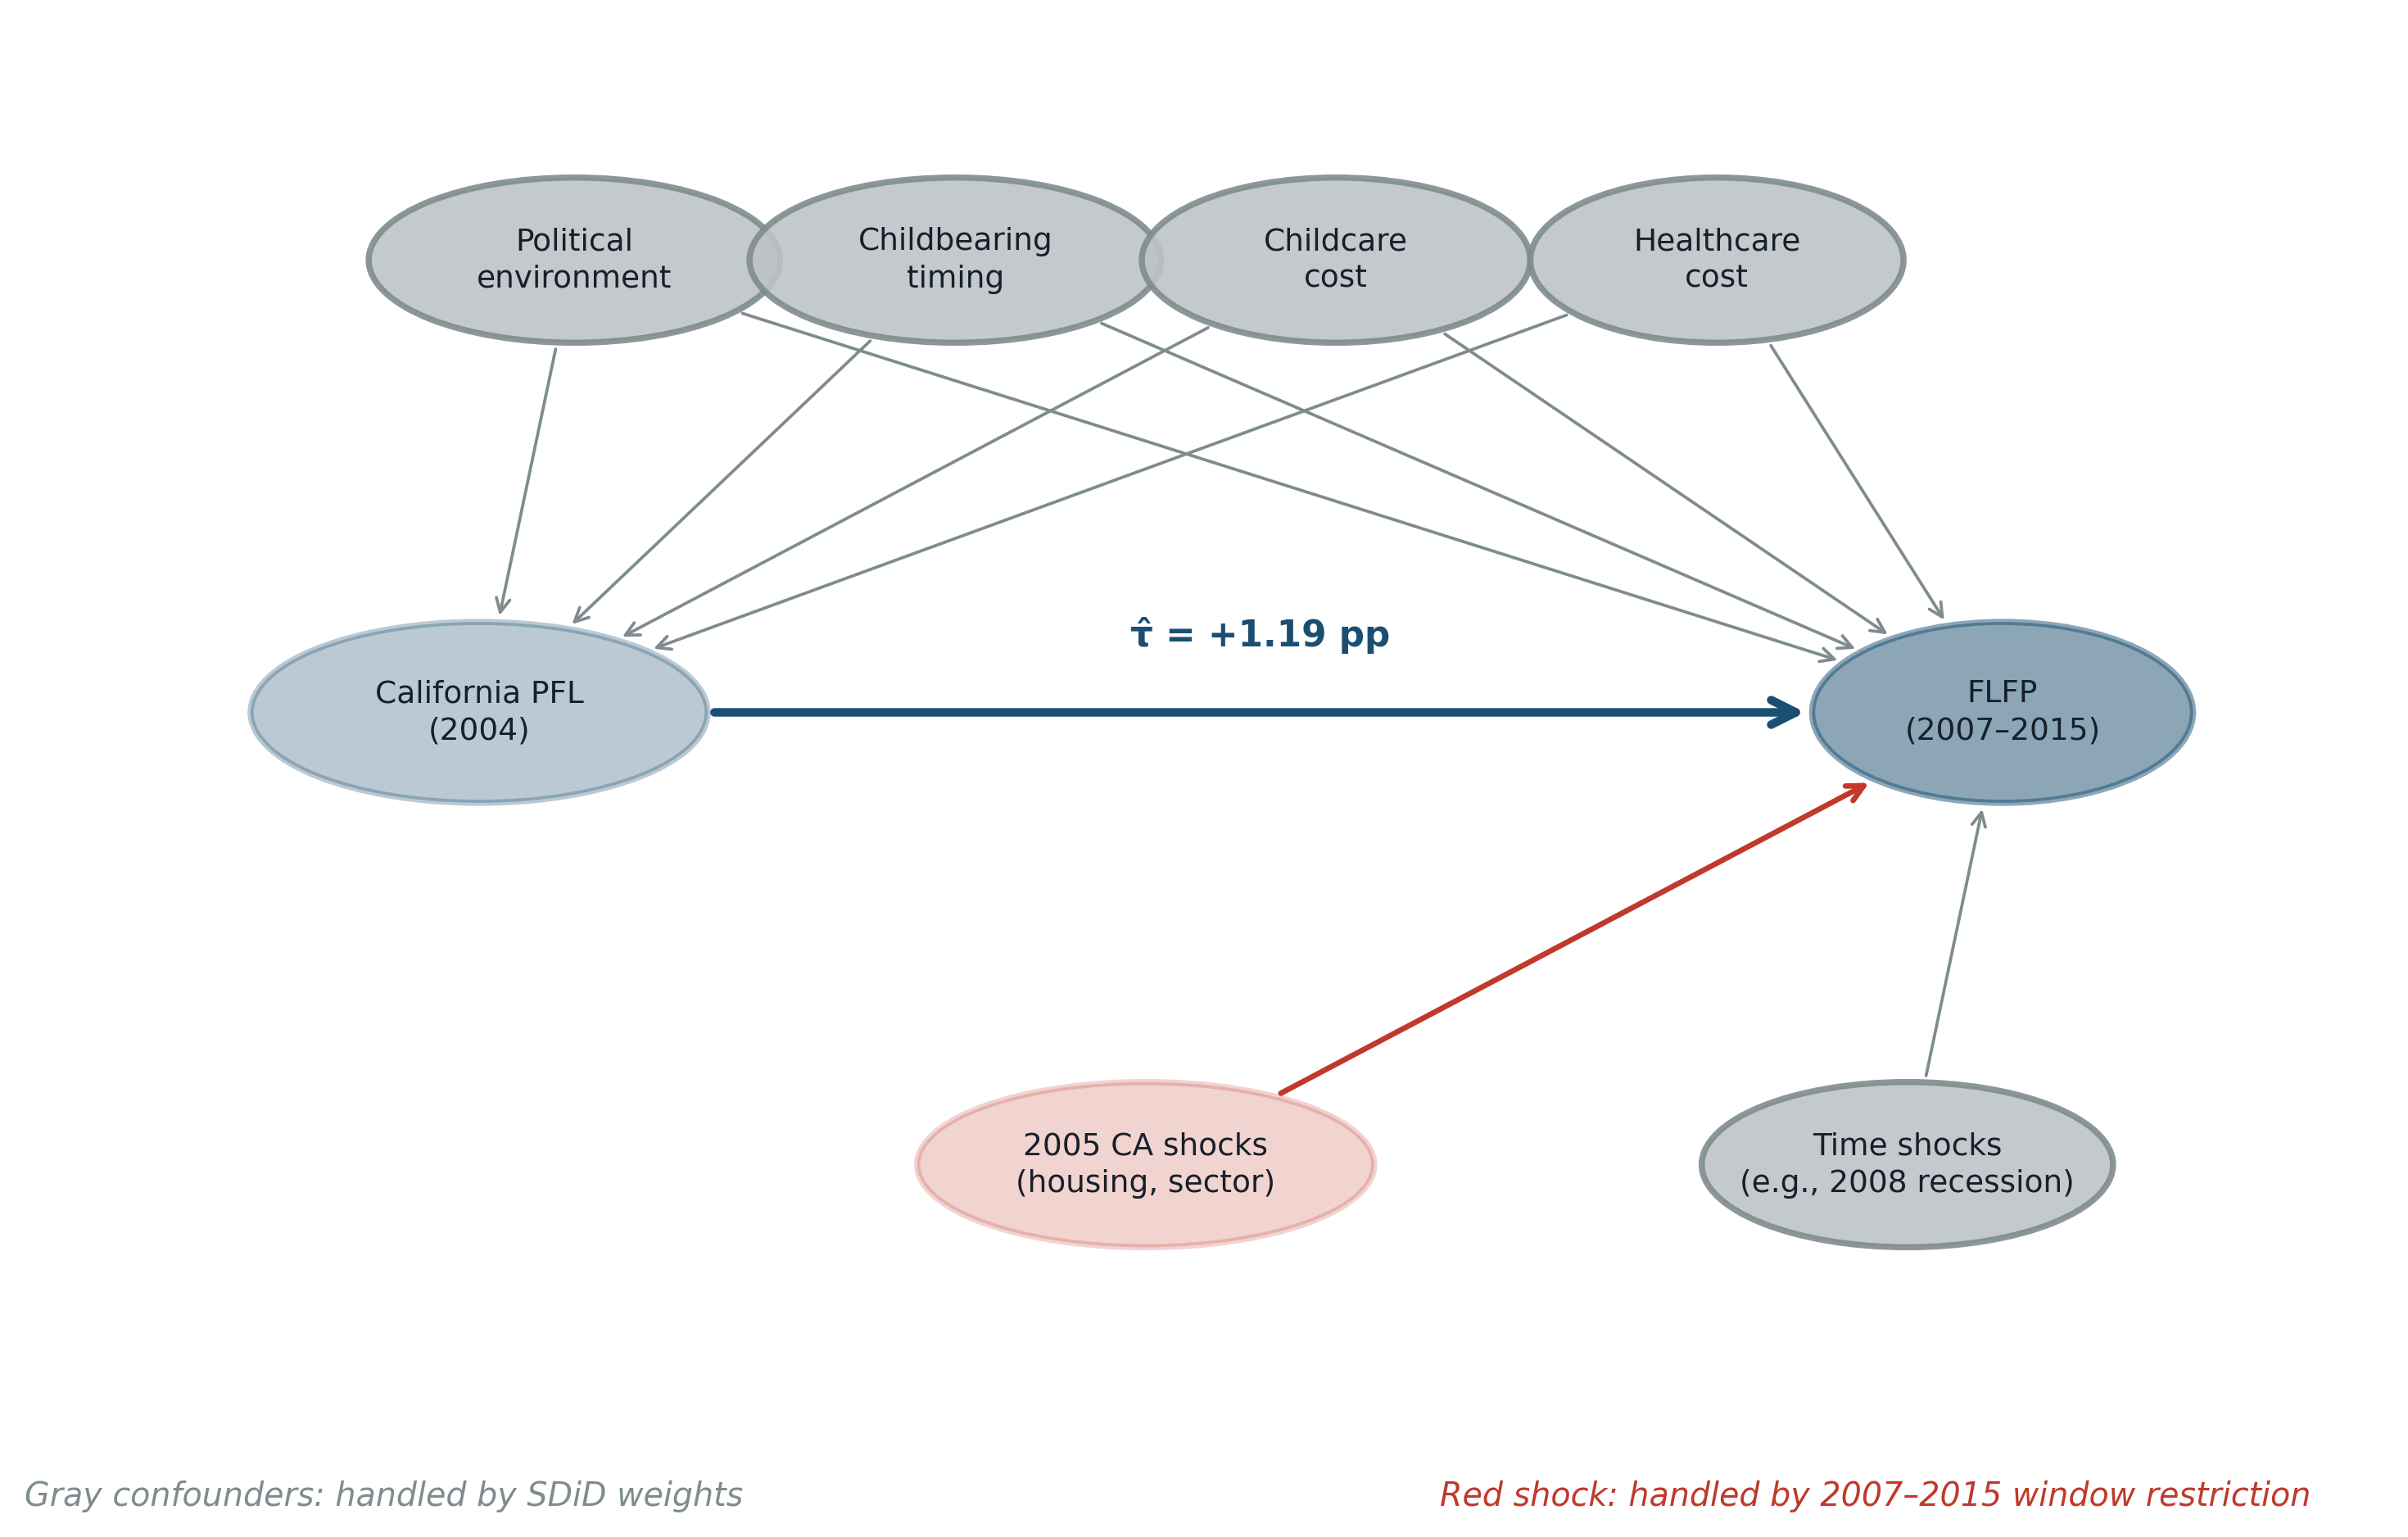
\includegraphics[width=0.99\textwidth]{pres_causal_dag.png}
\caption*{\footnotesize \textit{Notes:} Gray confounders are absorbed by the SDiD weighting scheme: unit weights match California's pre-treatment trajectory, and time weights identify informative pre-treatment years. The red node, 2005 California-specific shocks including housing wealth, immigration composition, and sectoral dynamics, is addressed by the 2007 to 2015 window restriction documented in Section 3.3.}
\end{figure}

\begin{figure}[H]
\centering
\caption{PFL Awareness Diffusion and Claims Growth, 2003 to 2015}
\label{fig:awareness}
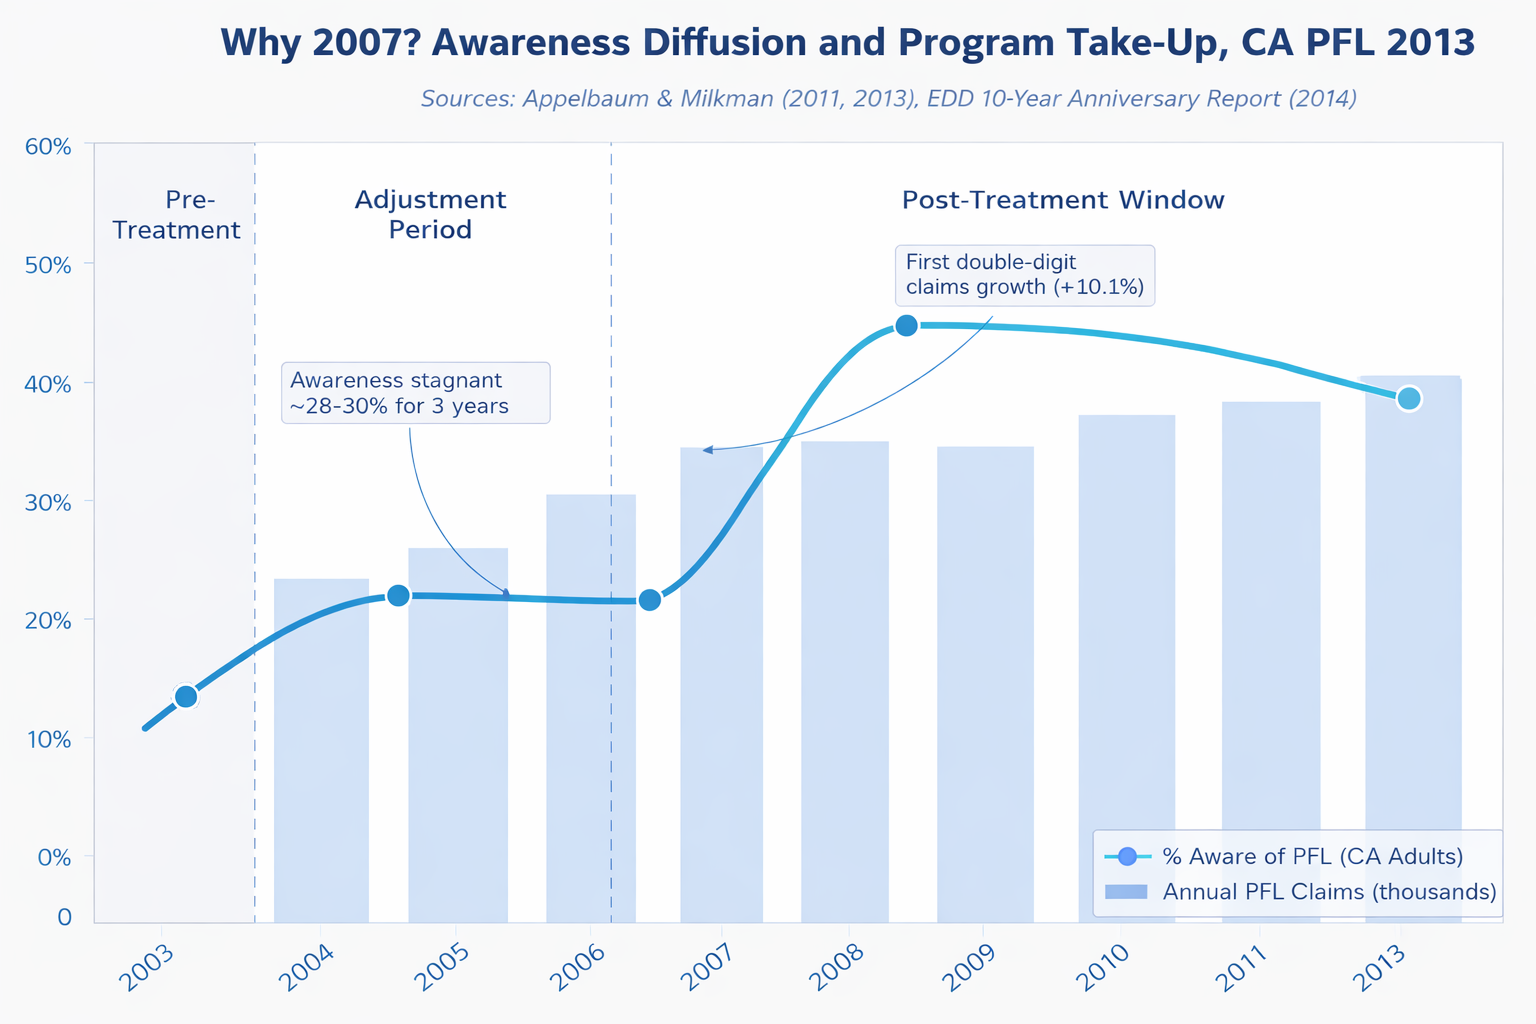
\includegraphics[width=0.95\textwidth]{pres_awareness_claims.png}
\caption*{\footnotesize \textit{Notes:} Awareness percentages from \citet{appelbaum2011} and the Golden Bear Omnibus Survey (UCLA, 2003). Claims data from the California Employment Development Department \citep{edd2014}. Fiscal year 2013--14 through 2015--16 claims values are interpolated from EDD chart data; precise tabular figures were not available for these years.}
\end{figure}

\begin{figure}[H]
\centering
\caption{In-Space Placebo Test, Synthetic DiD}
\label{fig:placebo}
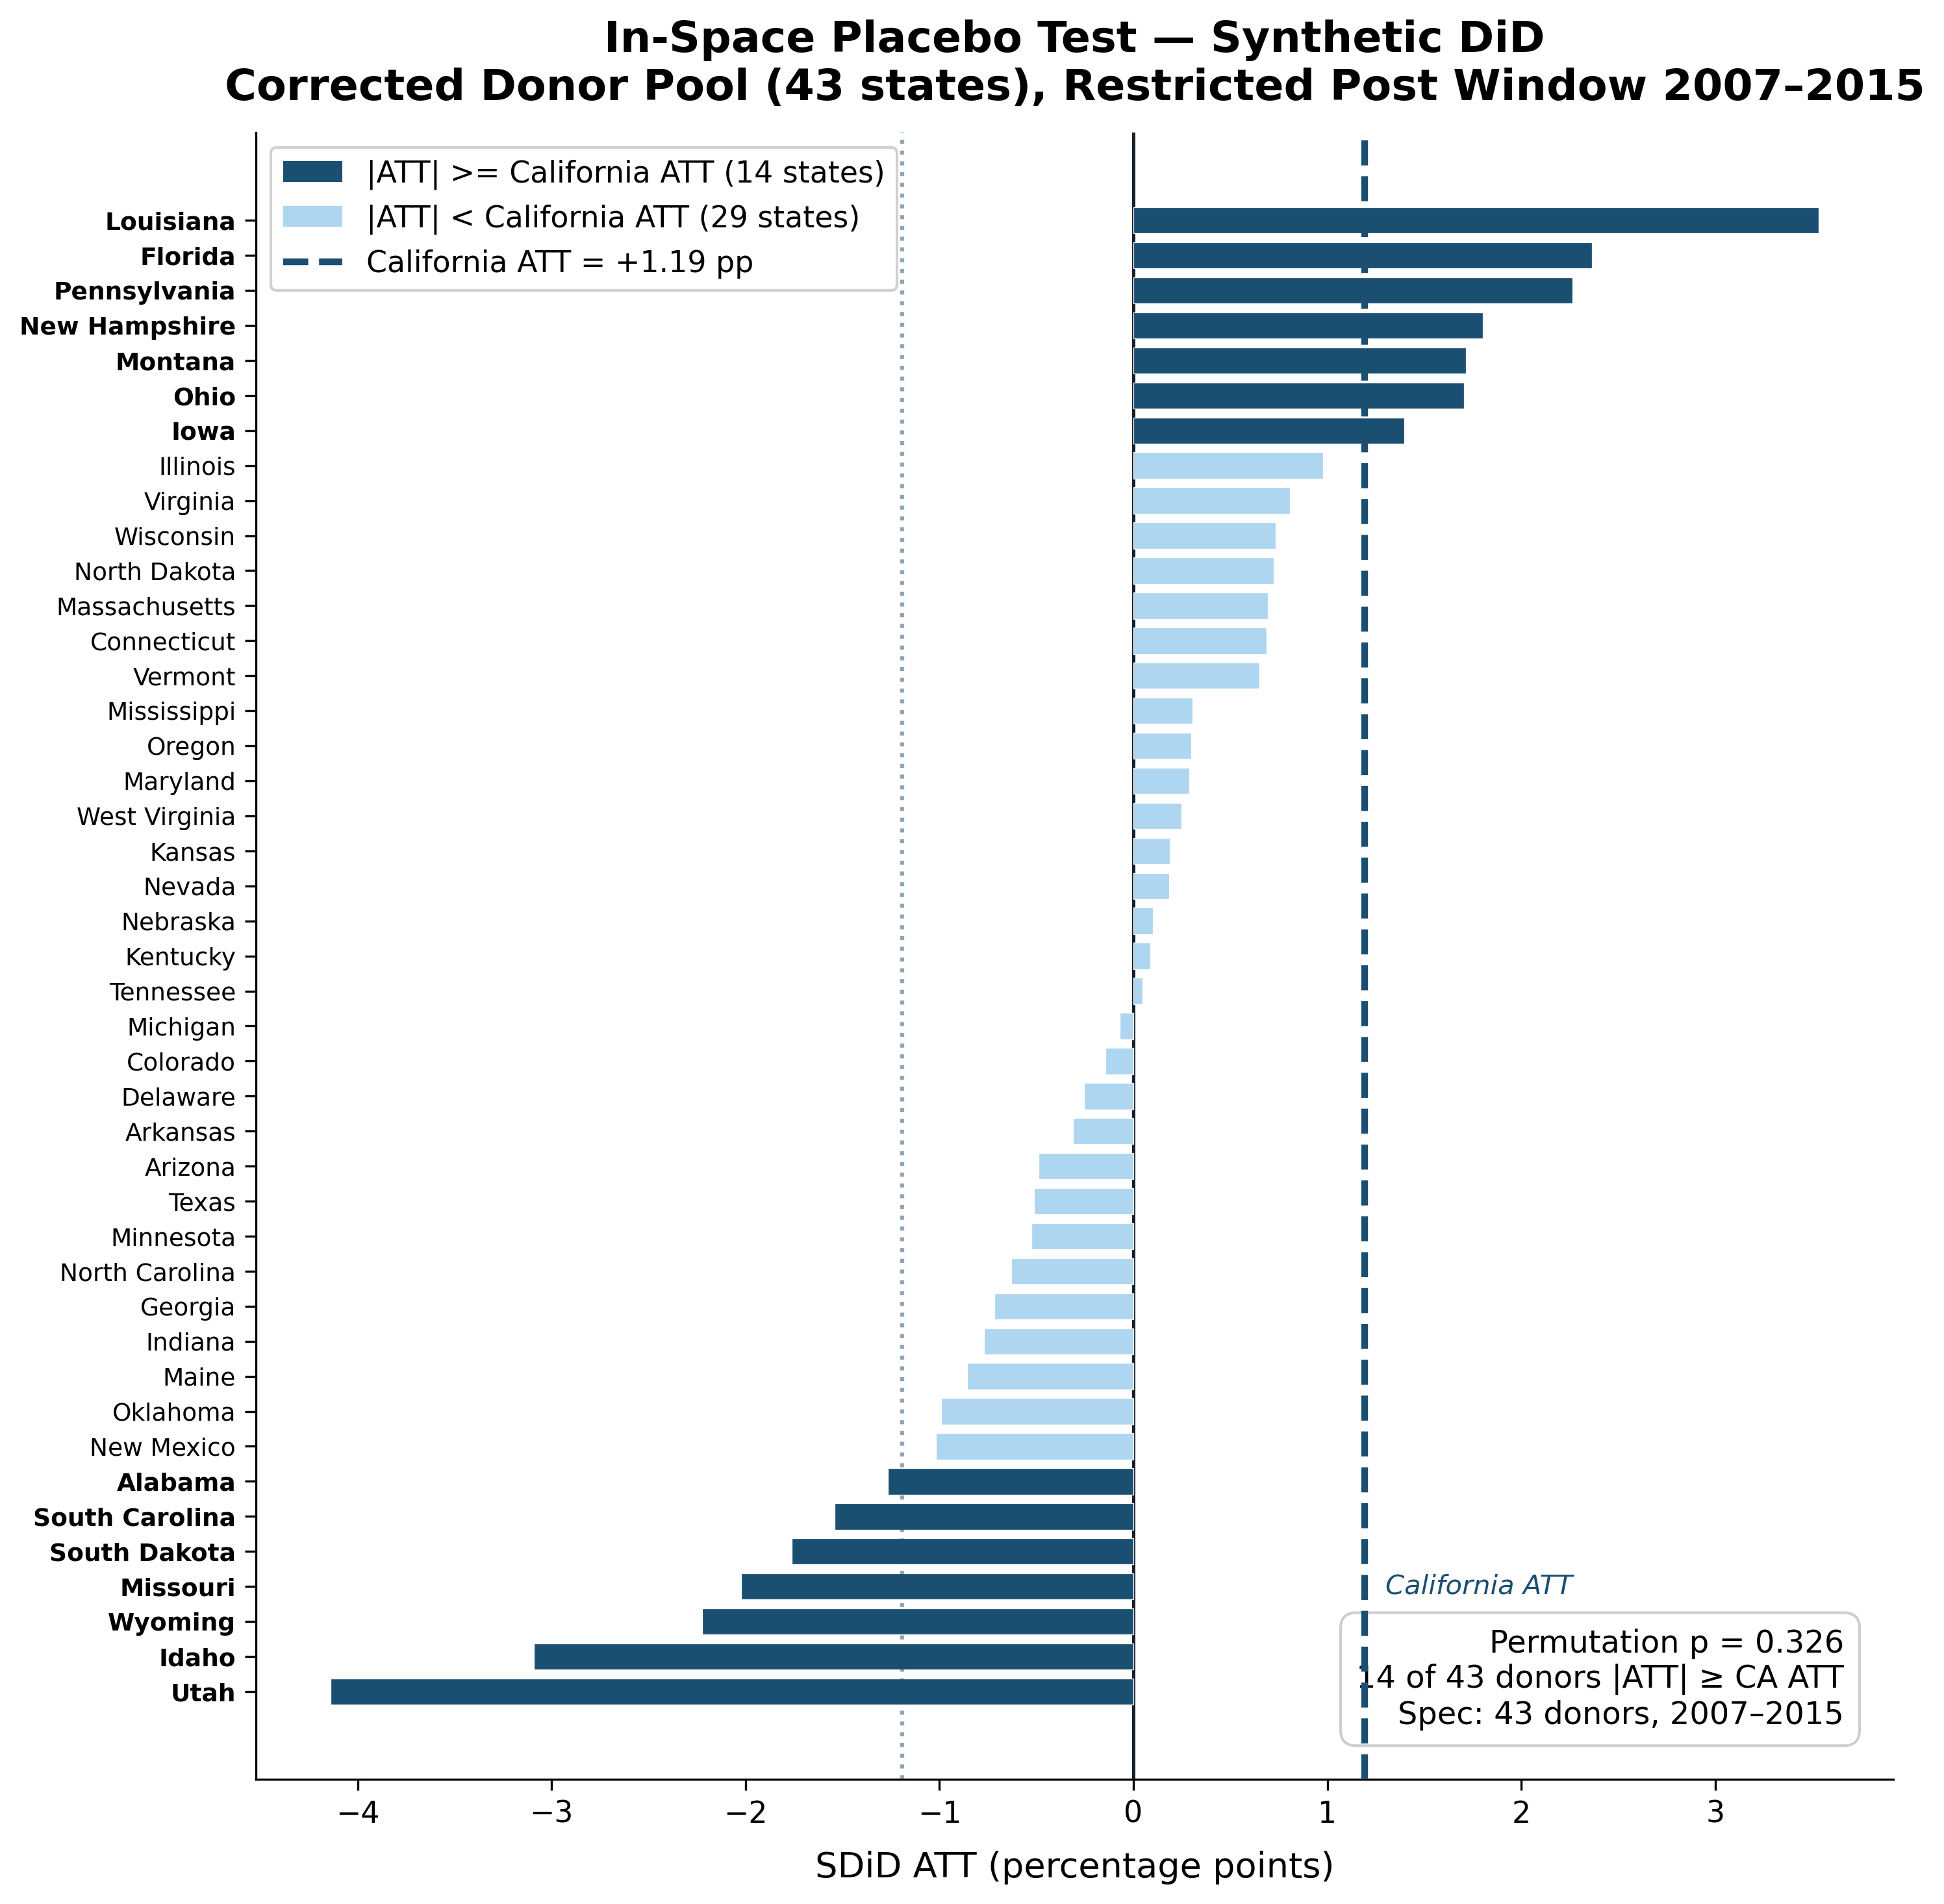
\includegraphics[width=0.75\textwidth]{pres_placebo.png}
\end{figure}

\begin{figure}[H]
\centering
\caption{Synthetic California Composition, SDiD Unit Weights}
\label{fig:weights}
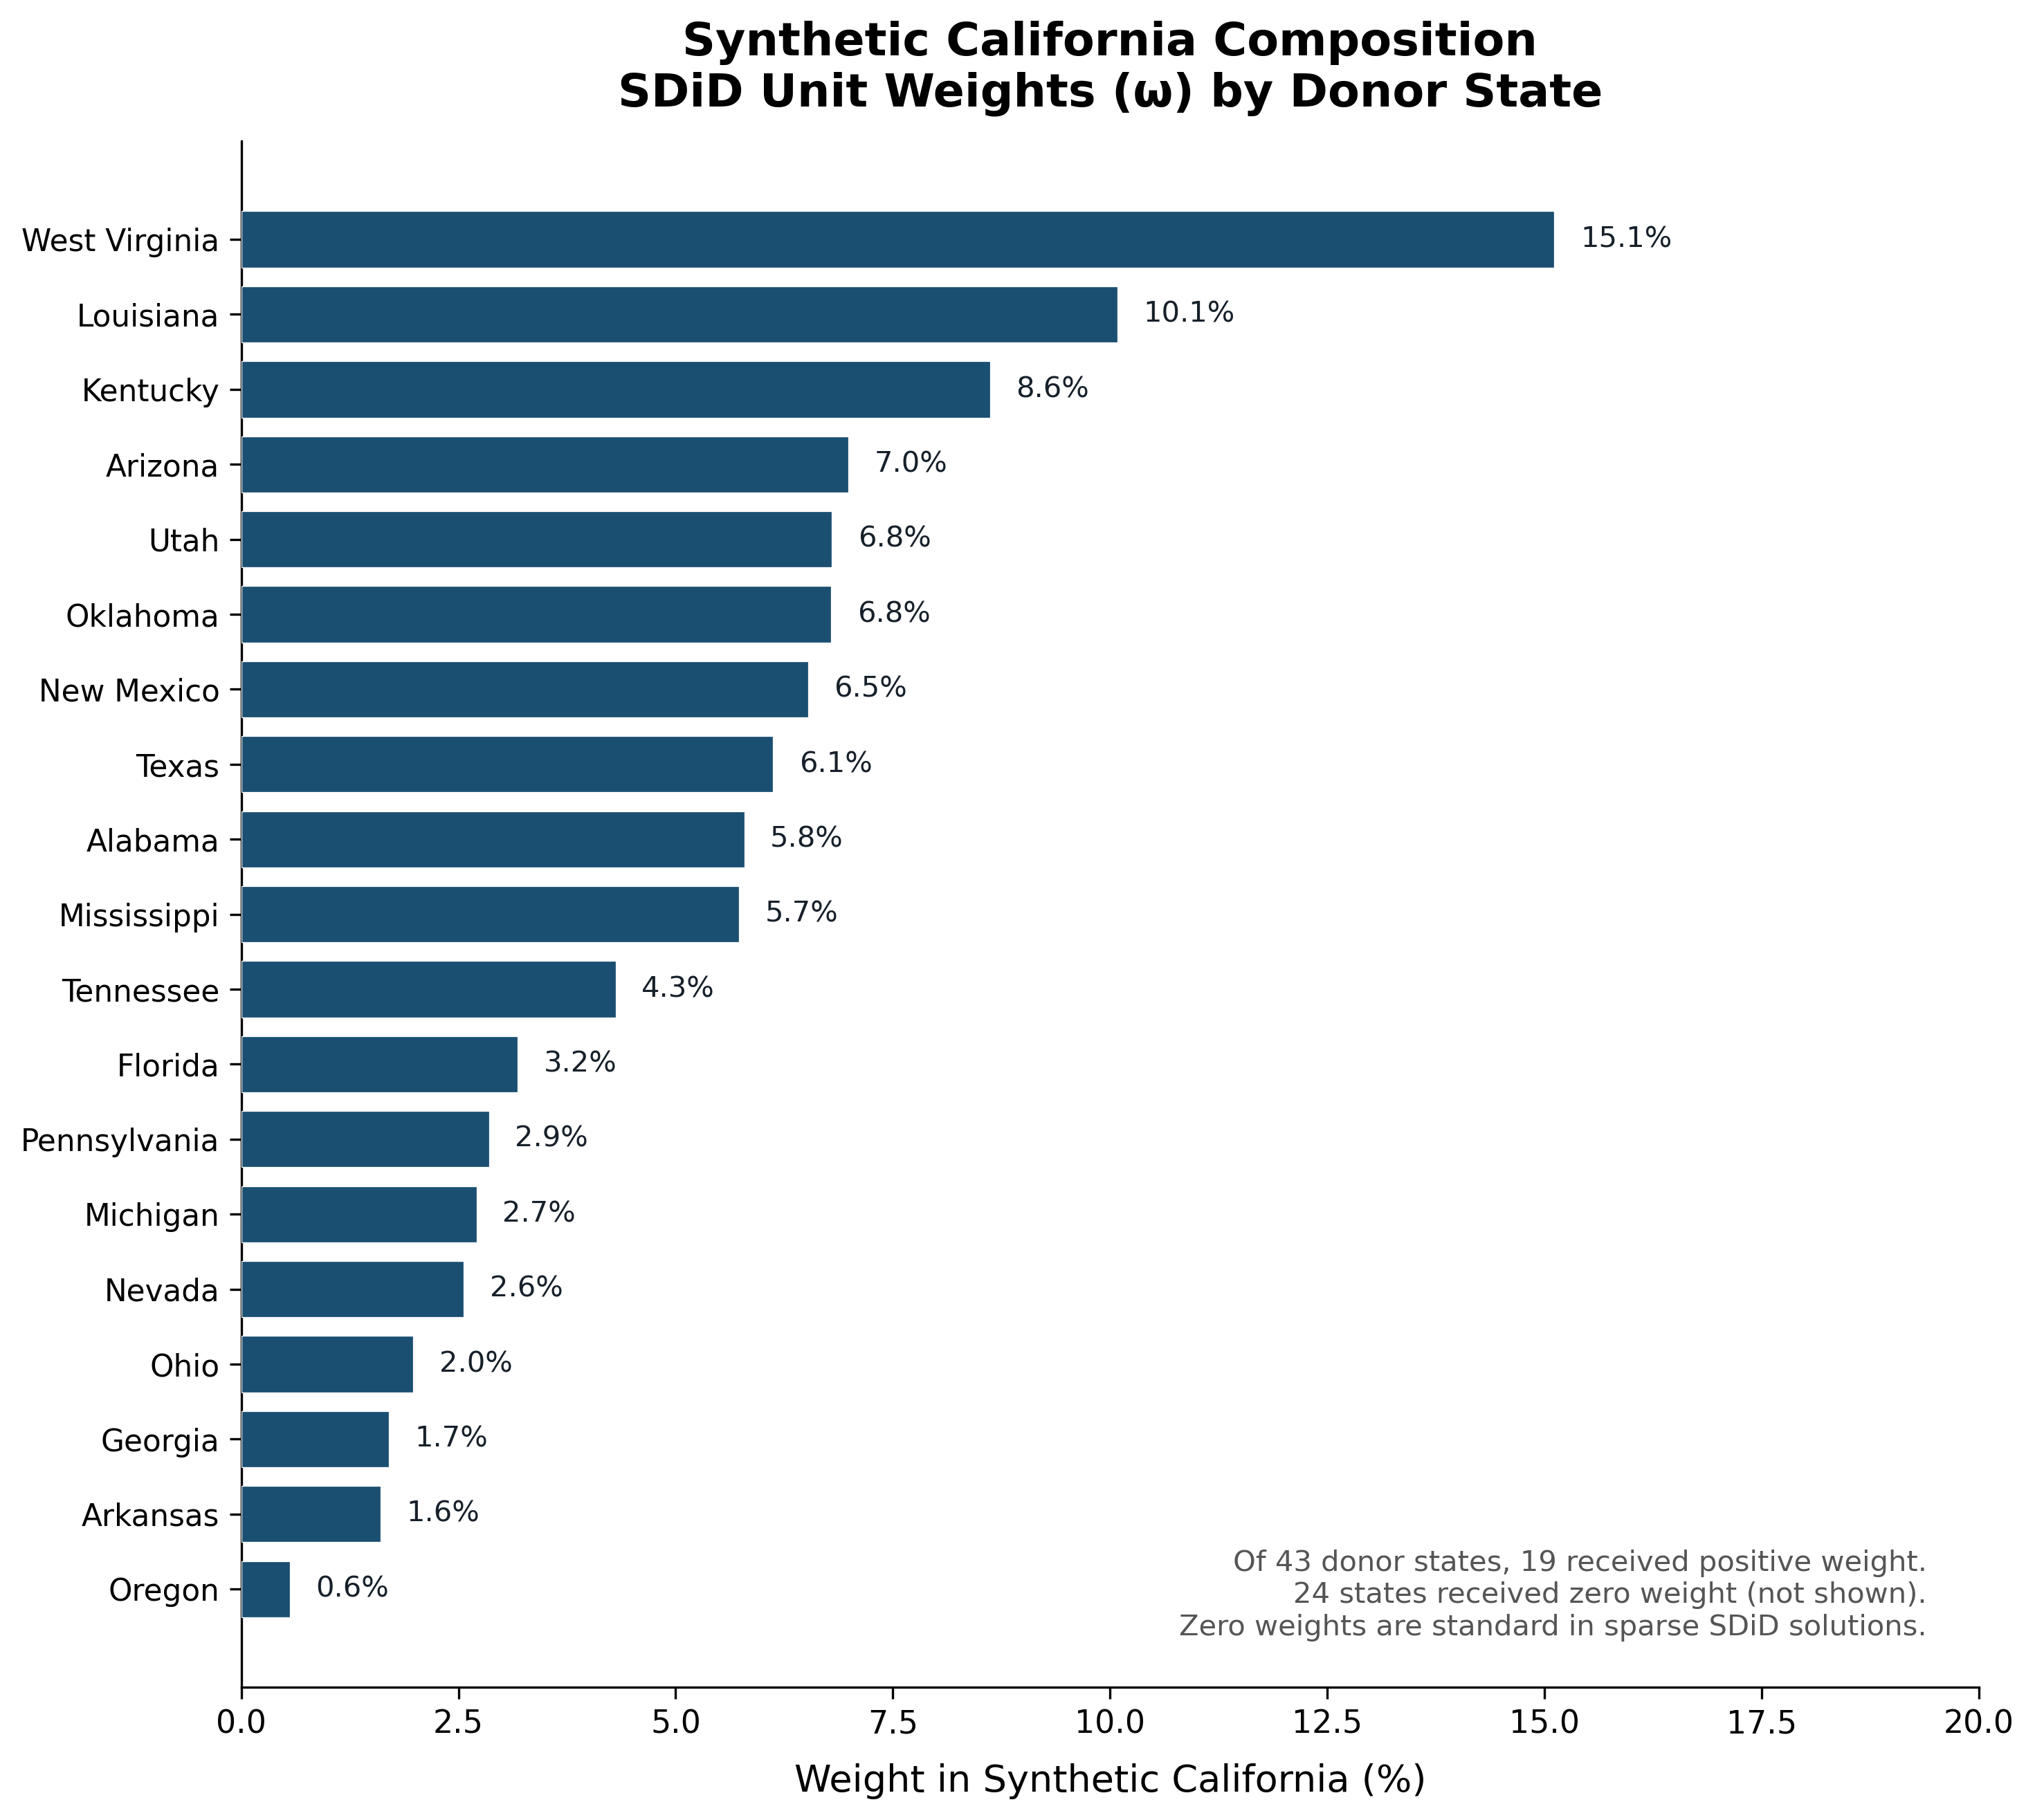
\includegraphics[width=0.80\textwidth]{pres_donor_weights.png}
\end{figure}

\begin{figure}[H]
\centering
\caption{Event Study Including 2004 to 2006 Adjustment Period}
\label{fig:eventstudyfull}
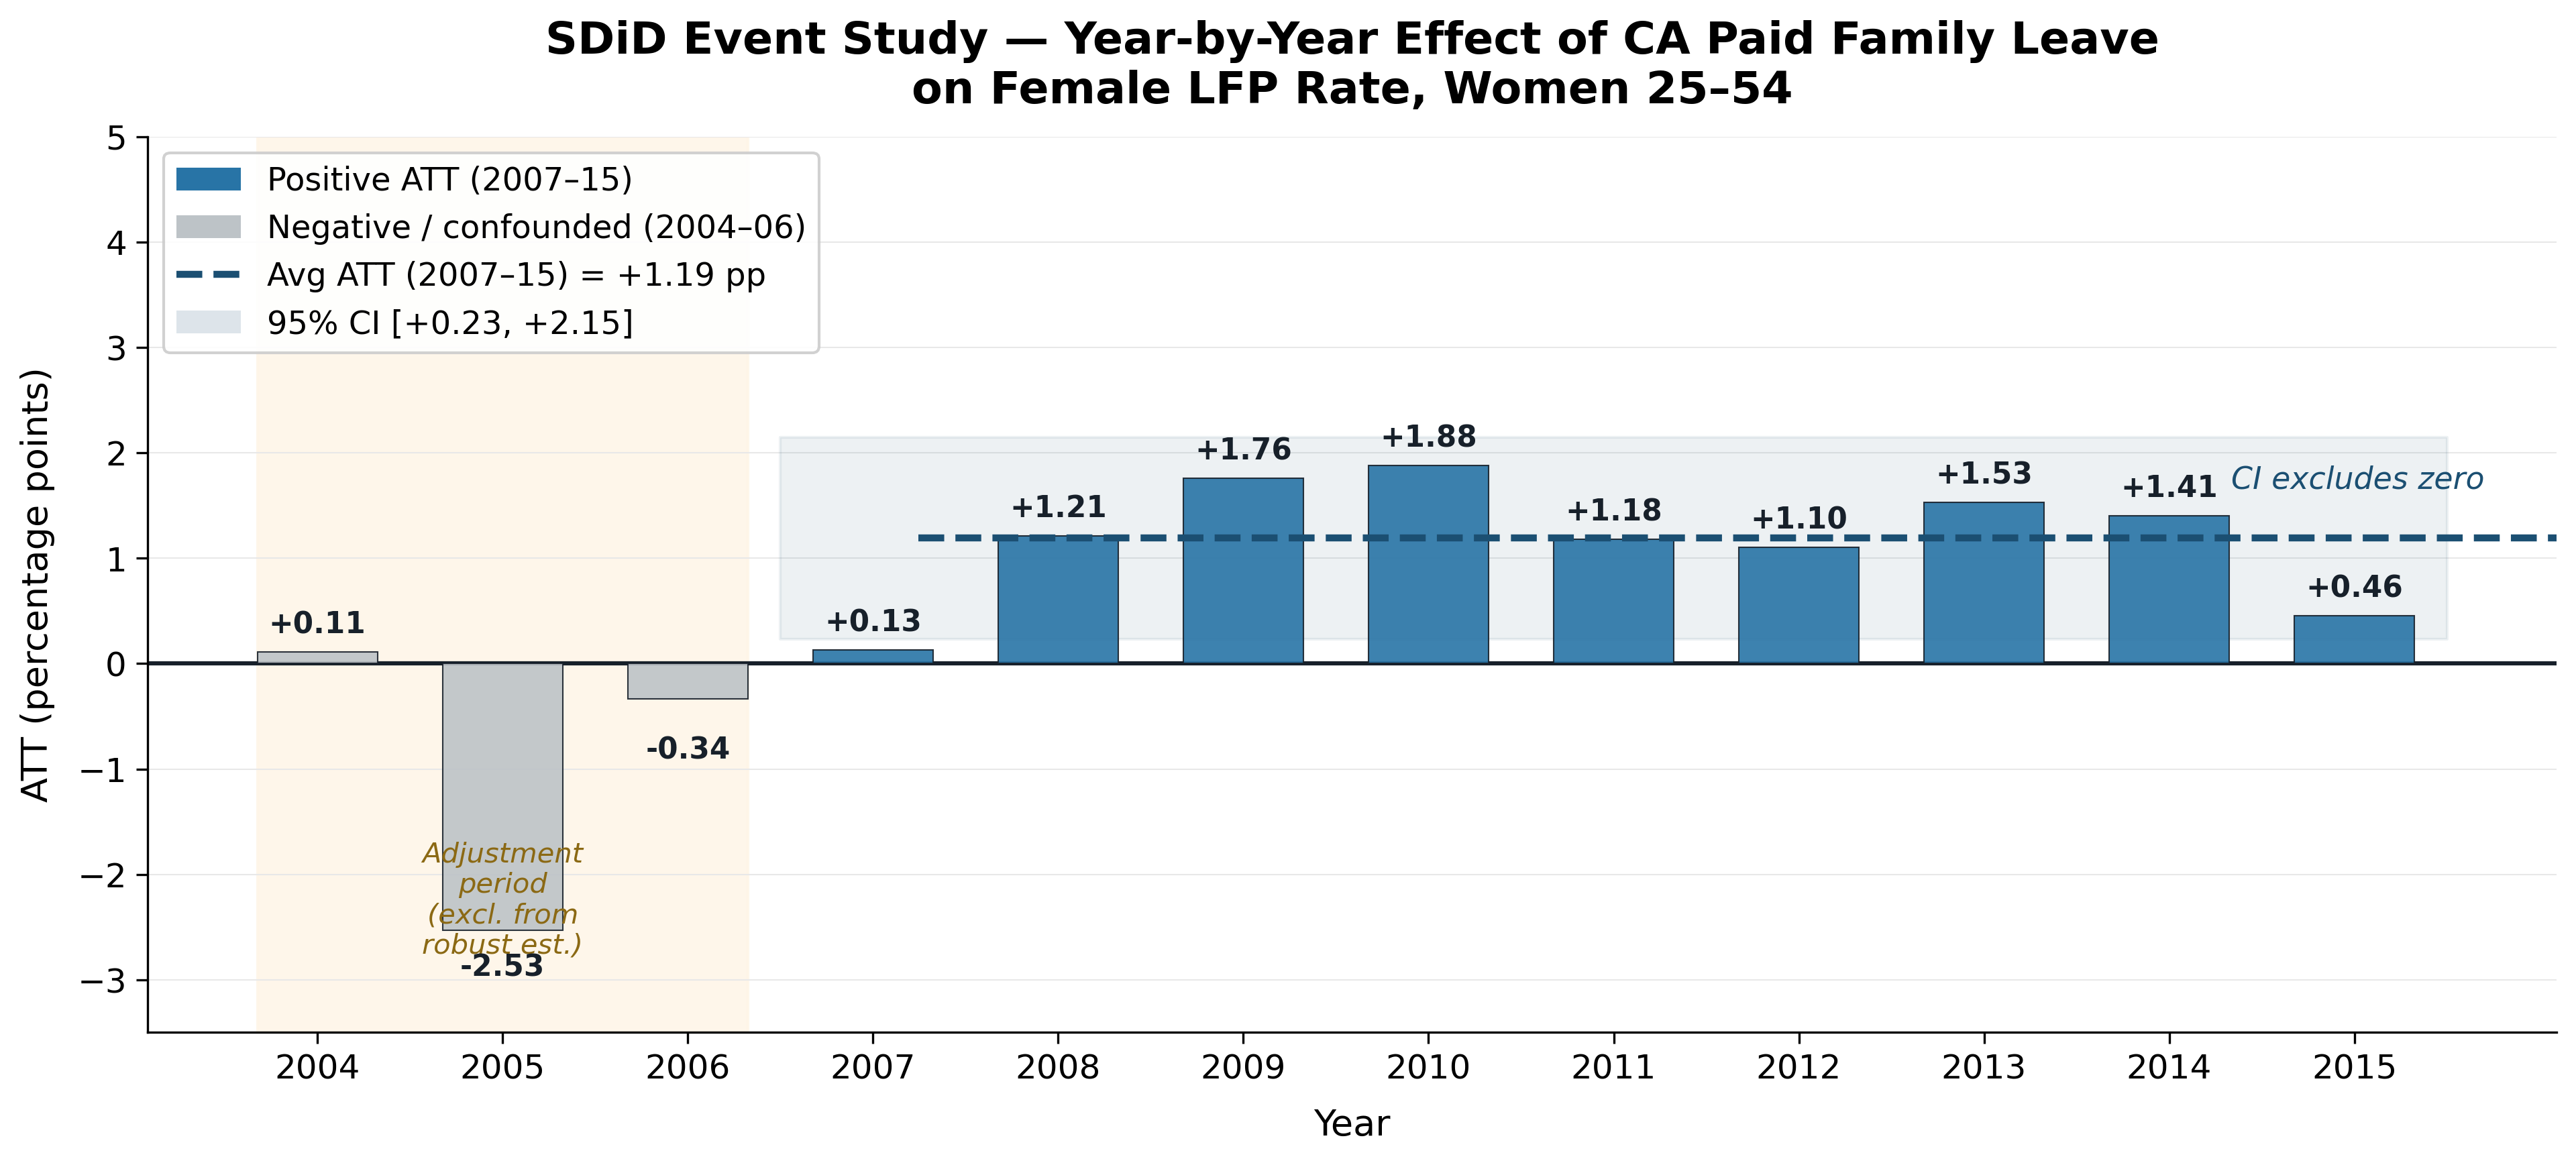
\includegraphics[width=0.90\textwidth]{pres_event_study.png}
\end{figure}

\begin{figure}[H]
\centering
\caption{Line Event Study}
\label{fig:eventstudyfull}
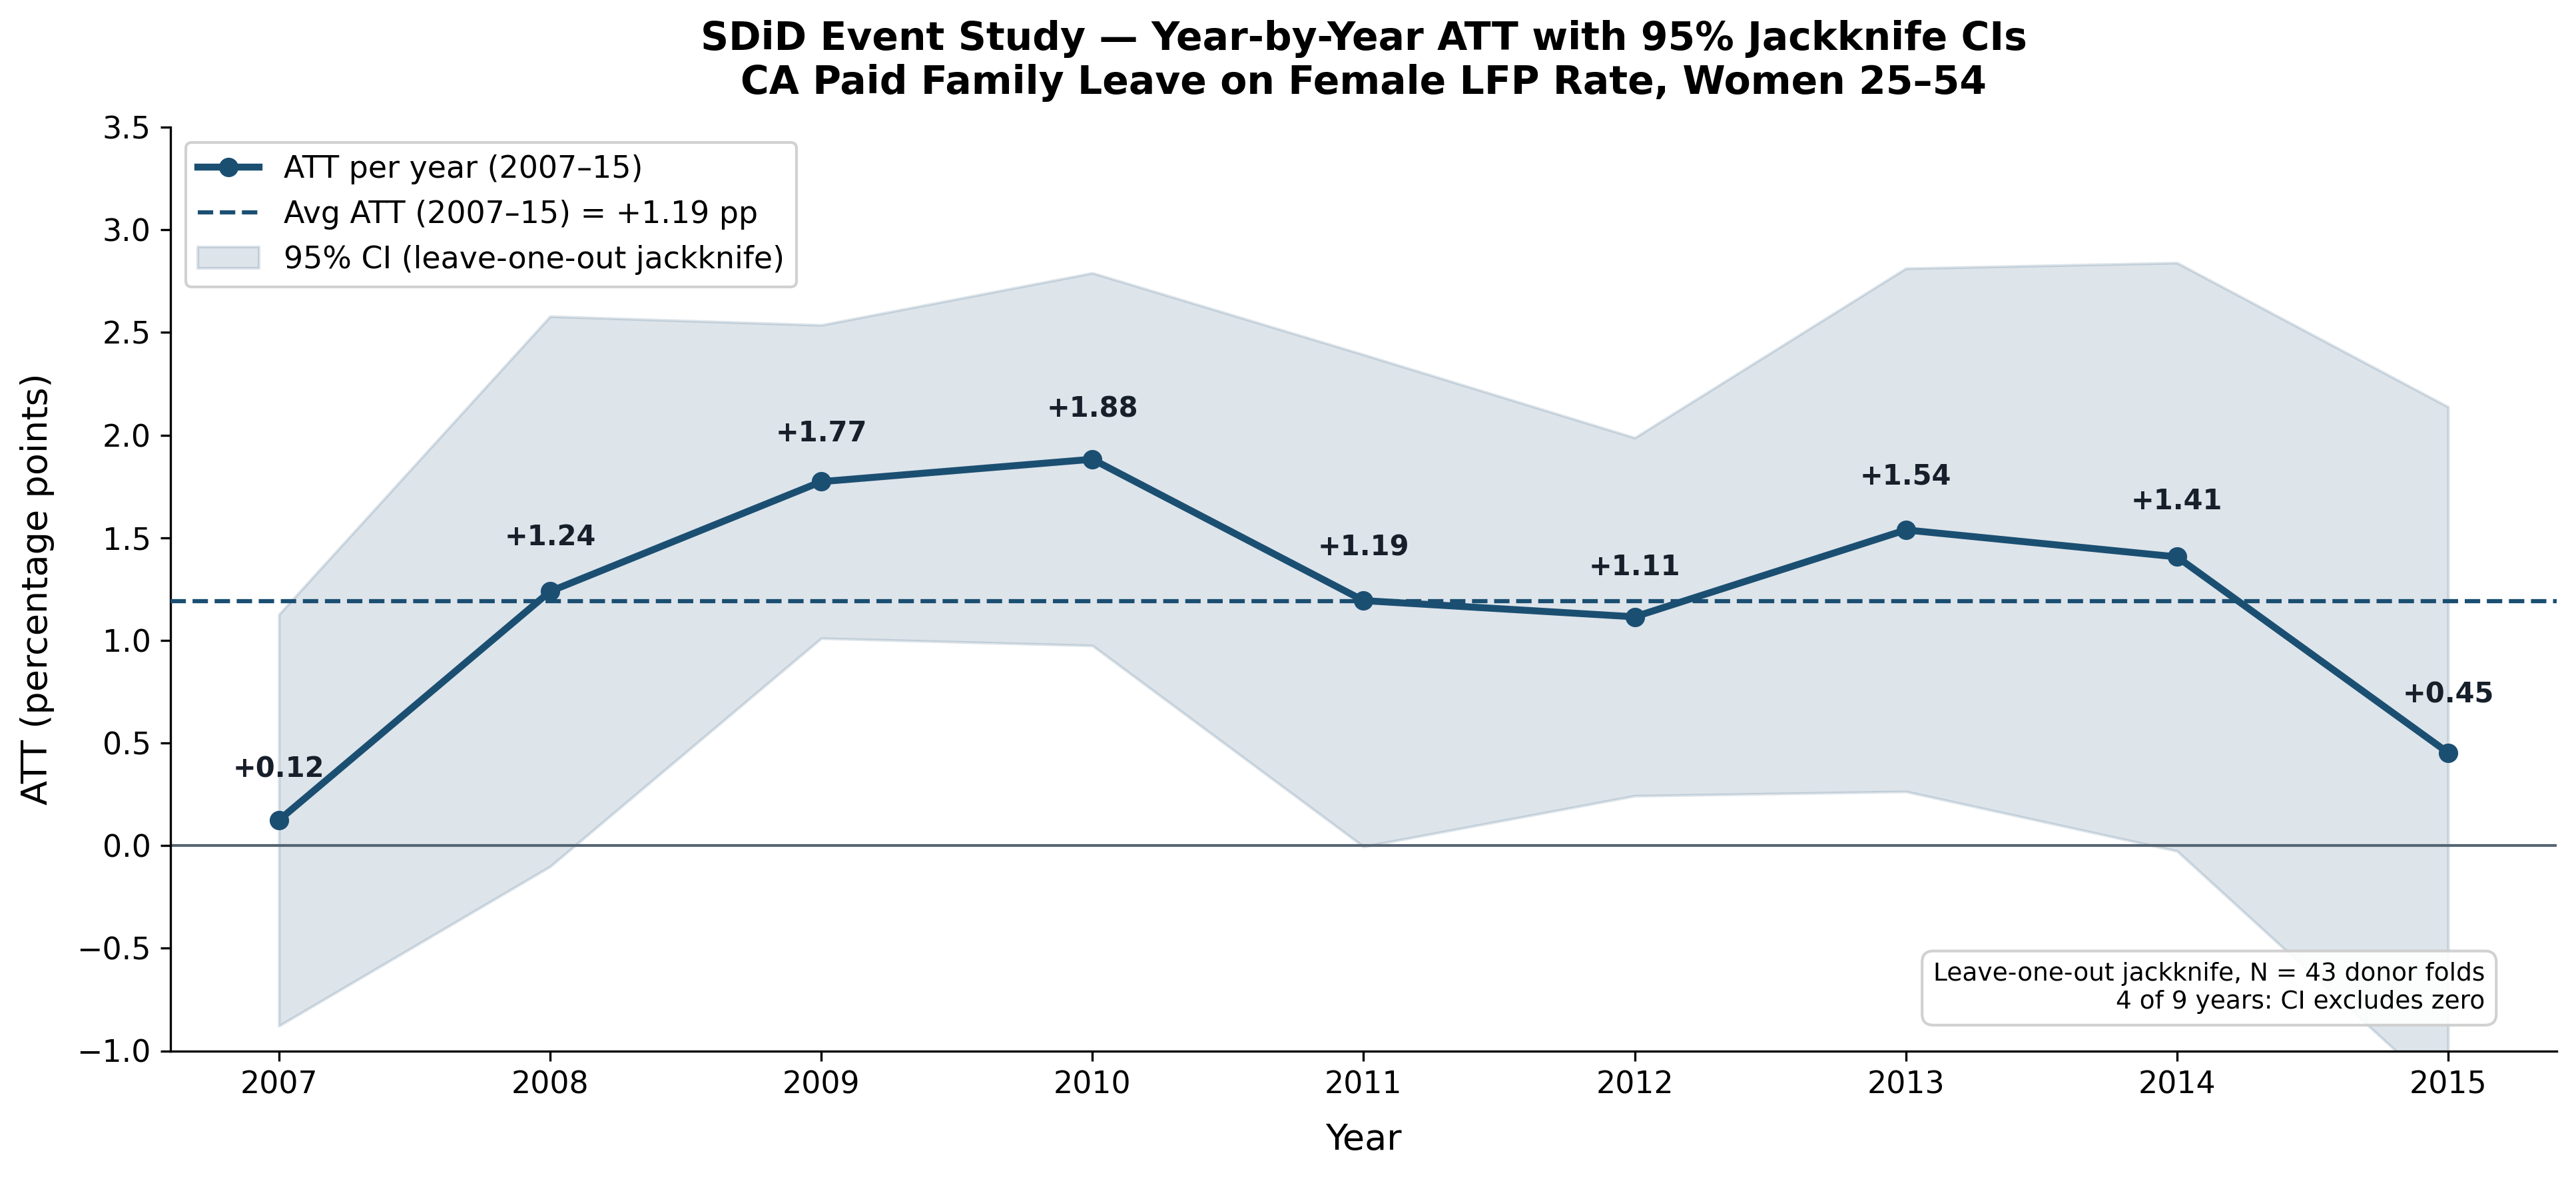
\includegraphics[width=0.90\textwidth]{pres_event_study_line.png}
\end{figure}

\begin{figure}[H]
\centering
\caption{Trend Plot with Zoomed Y-Axis (Truncated Range)}
\label{fig:trendzoom}
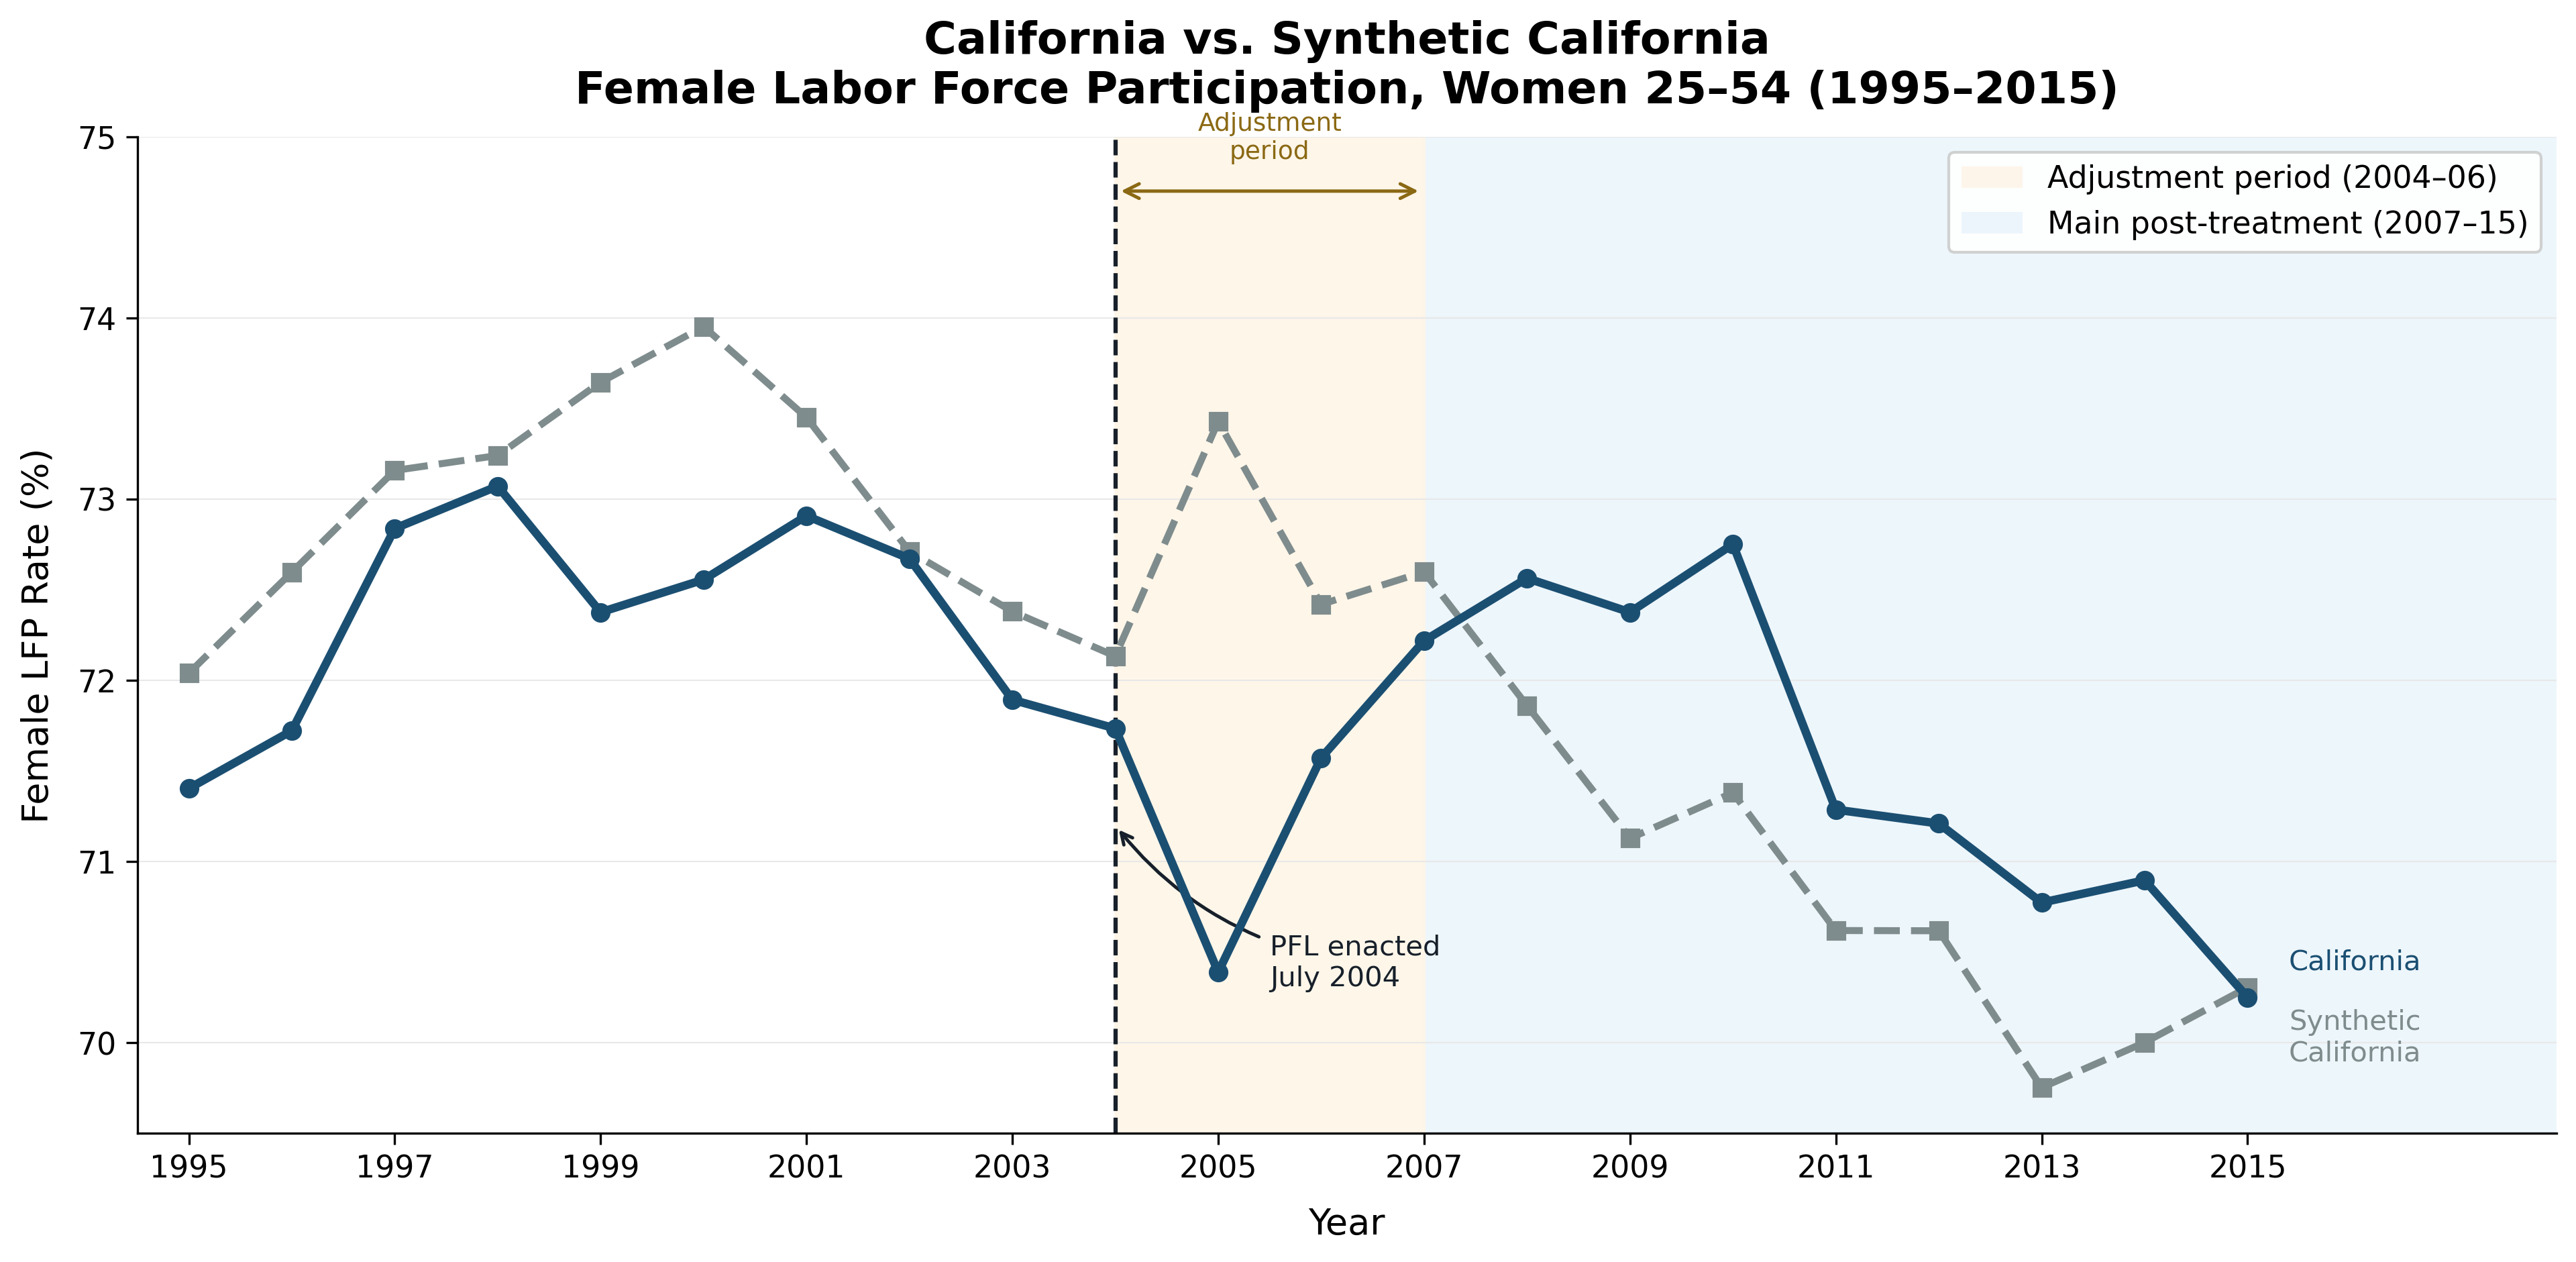
\includegraphics[width=0.95\textwidth]{pres_trend.png}
\caption*{\footnotesize \textit{Notes:} Alternative version of Figure \ref{fig:trend} with truncated y-axis to highlight post-treatment divergence. The main paper uses the context-axis version (40 to 80 percent range) to avoid visually exaggerating small differences.}
\end{figure}

\begin{figure}[H]
\centering
\caption{Pre-Treatment Fit with Zoomed Y-Axis (Truncated Range)}
\label{fig:pretrendzoom}
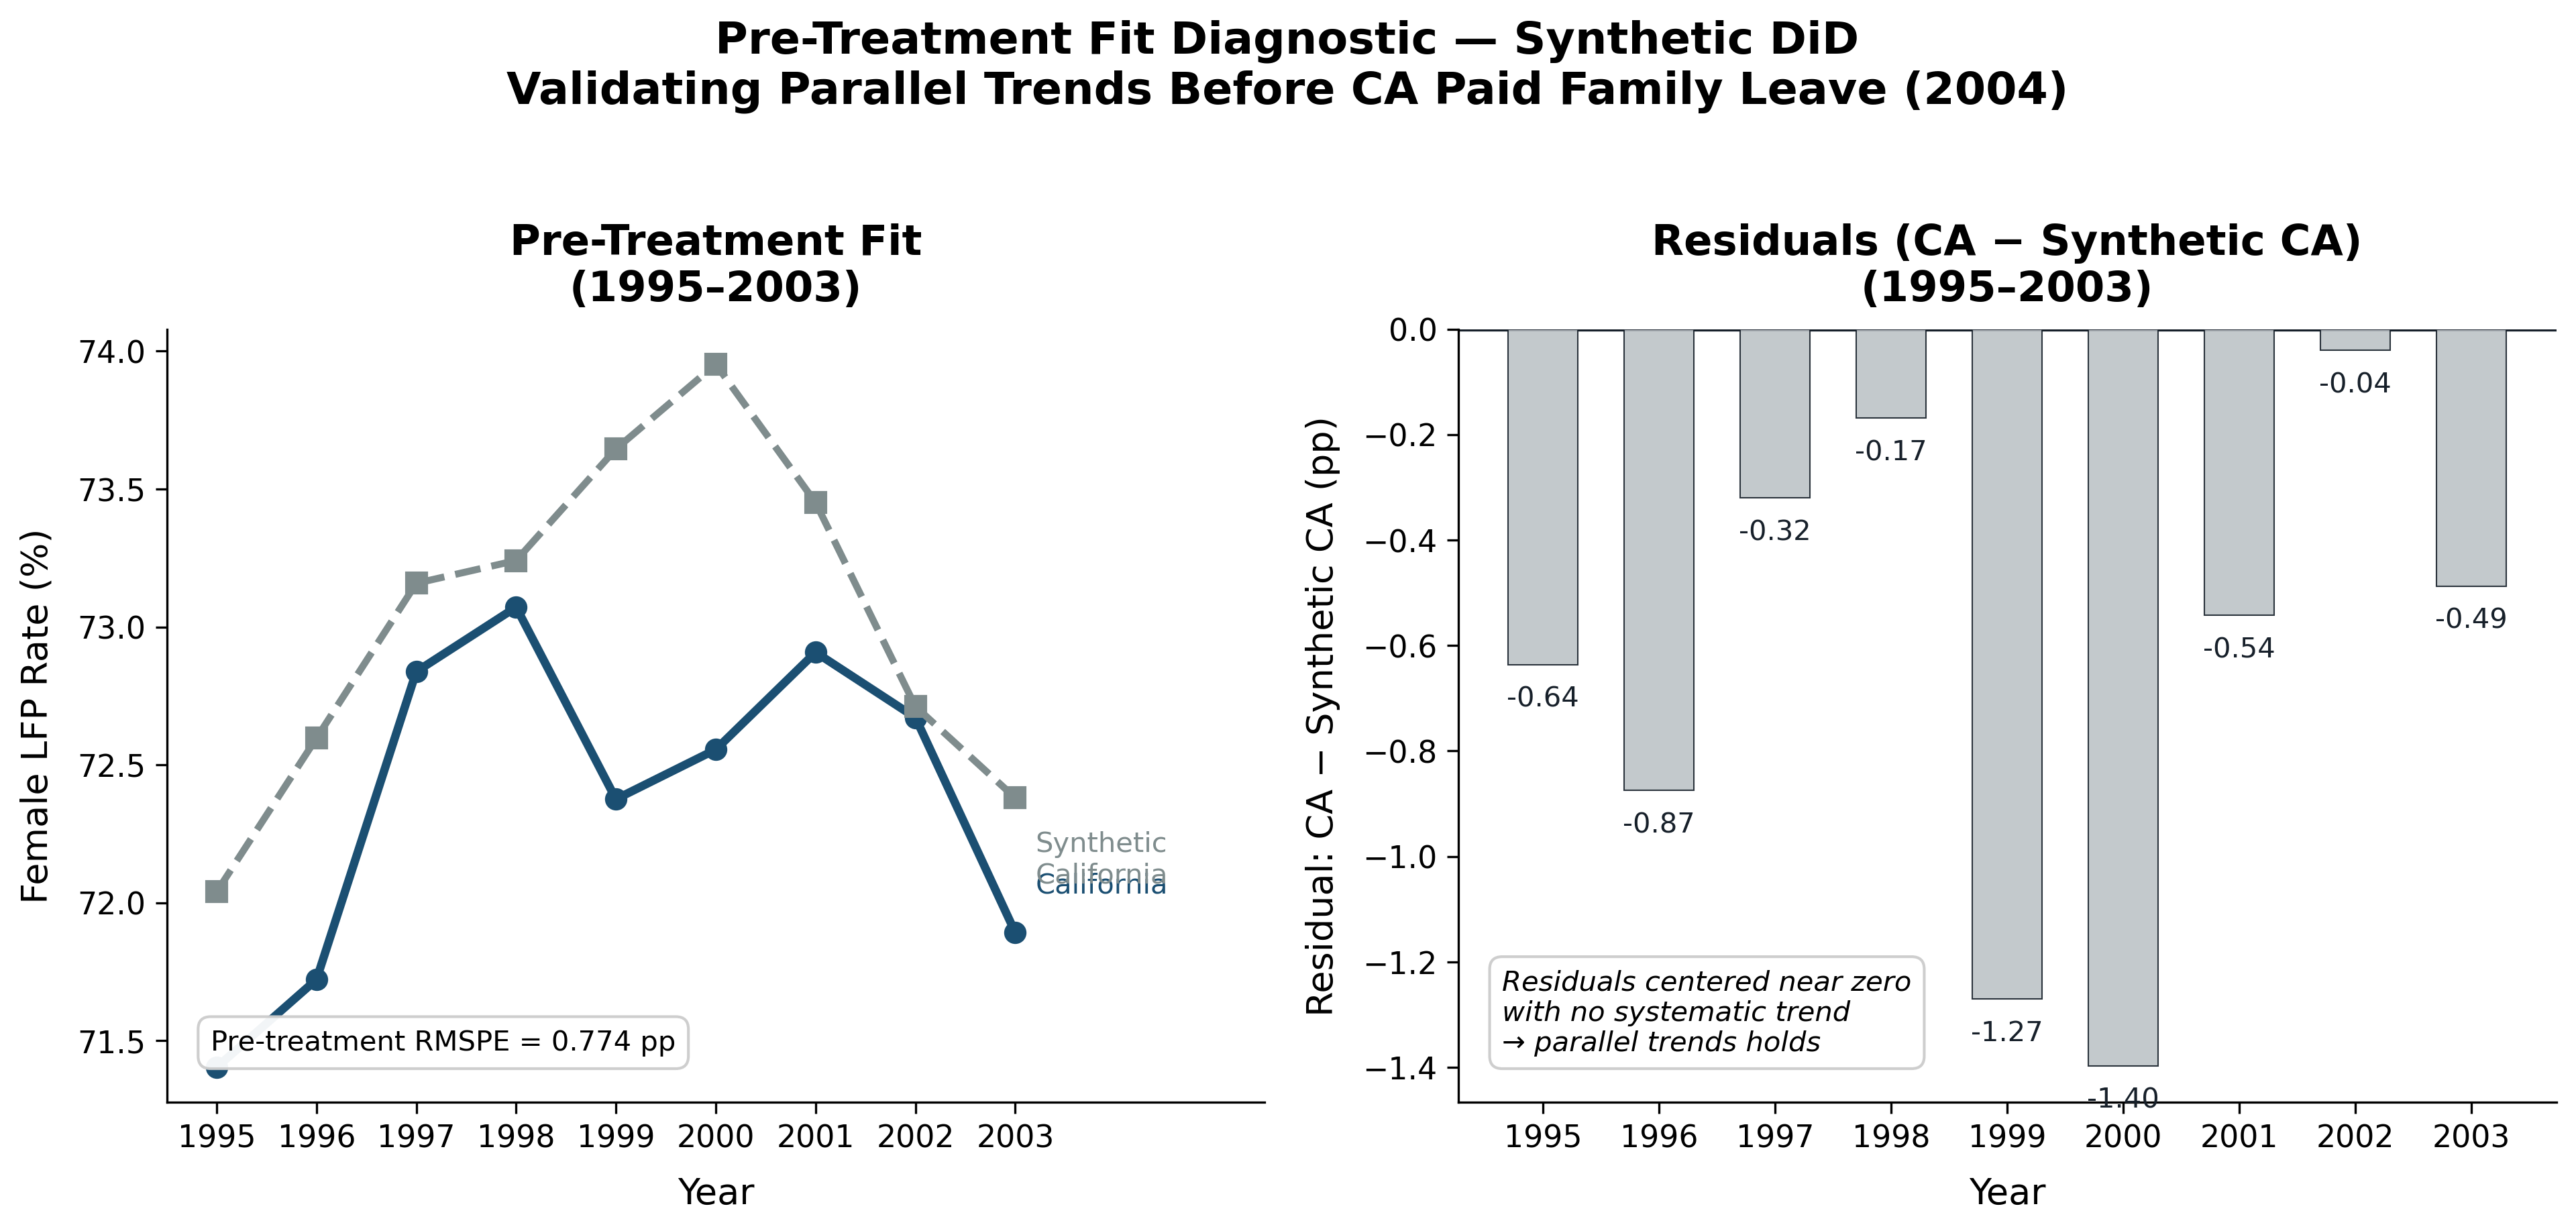
\includegraphics[width=0.95\textwidth]{pres_pretrend.png}
\caption*{\footnotesize \textit{Notes:} Alternative version of Figure \ref{fig:pretrend} with truncated y-axis. The main paper uses the context-axis version (40 to 80 percent range).}
\end{figure}

\end{document}